\chapter{Build-Measure-Learn}
\label{chap:results}

The following chapter presents the results of the project, as well as serving as a summary of the process dictated by Eric Ries' Build-Measure-Learn feedback loop \cite{lean_startup}. The chapter is divided into three main sections: one for each stage of the iterative process. The Build section showcases the resulting frontend application, or essentially the product of the project's final \textit{build} iteration. The Measure section presents a technical performance evaluation, as well as the results of the workshop held with the Roskilde Festival safety team. The latter also serves as a representation of the preceding \textit{measure} phases, where the product was presented to the safety team for feedback. Finally, the Learn section reflects on the value of the product, as well as assessing its fulfillment of the requirements outlined in previous chapters, representative of the evaluation conducted in each \textit{learn} phase.

\section{Build}
\label{sec:frontend-showcase}

Following the Build-Measure-Learn framework, the application was developed iteratively, with each version being refined based on user feedback. The process started with an extended Learn phase, where many conversations were held with the safety team in order to thoroughly grasp their needs and existing workflows. The product's first version was then built (Build), and Roskilde Festival's Mads and Morten Therkildsen were subsequently invited to provide feedback. Feedback in this case is the qualitative data netted from the Measure phase. This feedback was then analyzed and used to define new features and refine the product, which was then again presented and evaluated. The process was repeated until the final version was reached, which was presented in the workshop outlined in Section \ref{sec:business-value}.

This section showcases the resulting frontend application, which serves as the primary interface for the Roskilde Festival safety team to access and analyze crowd dynamics data. The interface is designed to be intuitive, presenting complex data through interactive charts and maps. The following figures illustrate the key features and functionalities of the application. Note that data shown from June 30th to July 2nd corresponds to the Eos stage, while data from July 3rd onwards corresponds to the Arena stage, as noted in Section \ref{sec:data_collection}.


\begin{figure}[H]
  \centering
  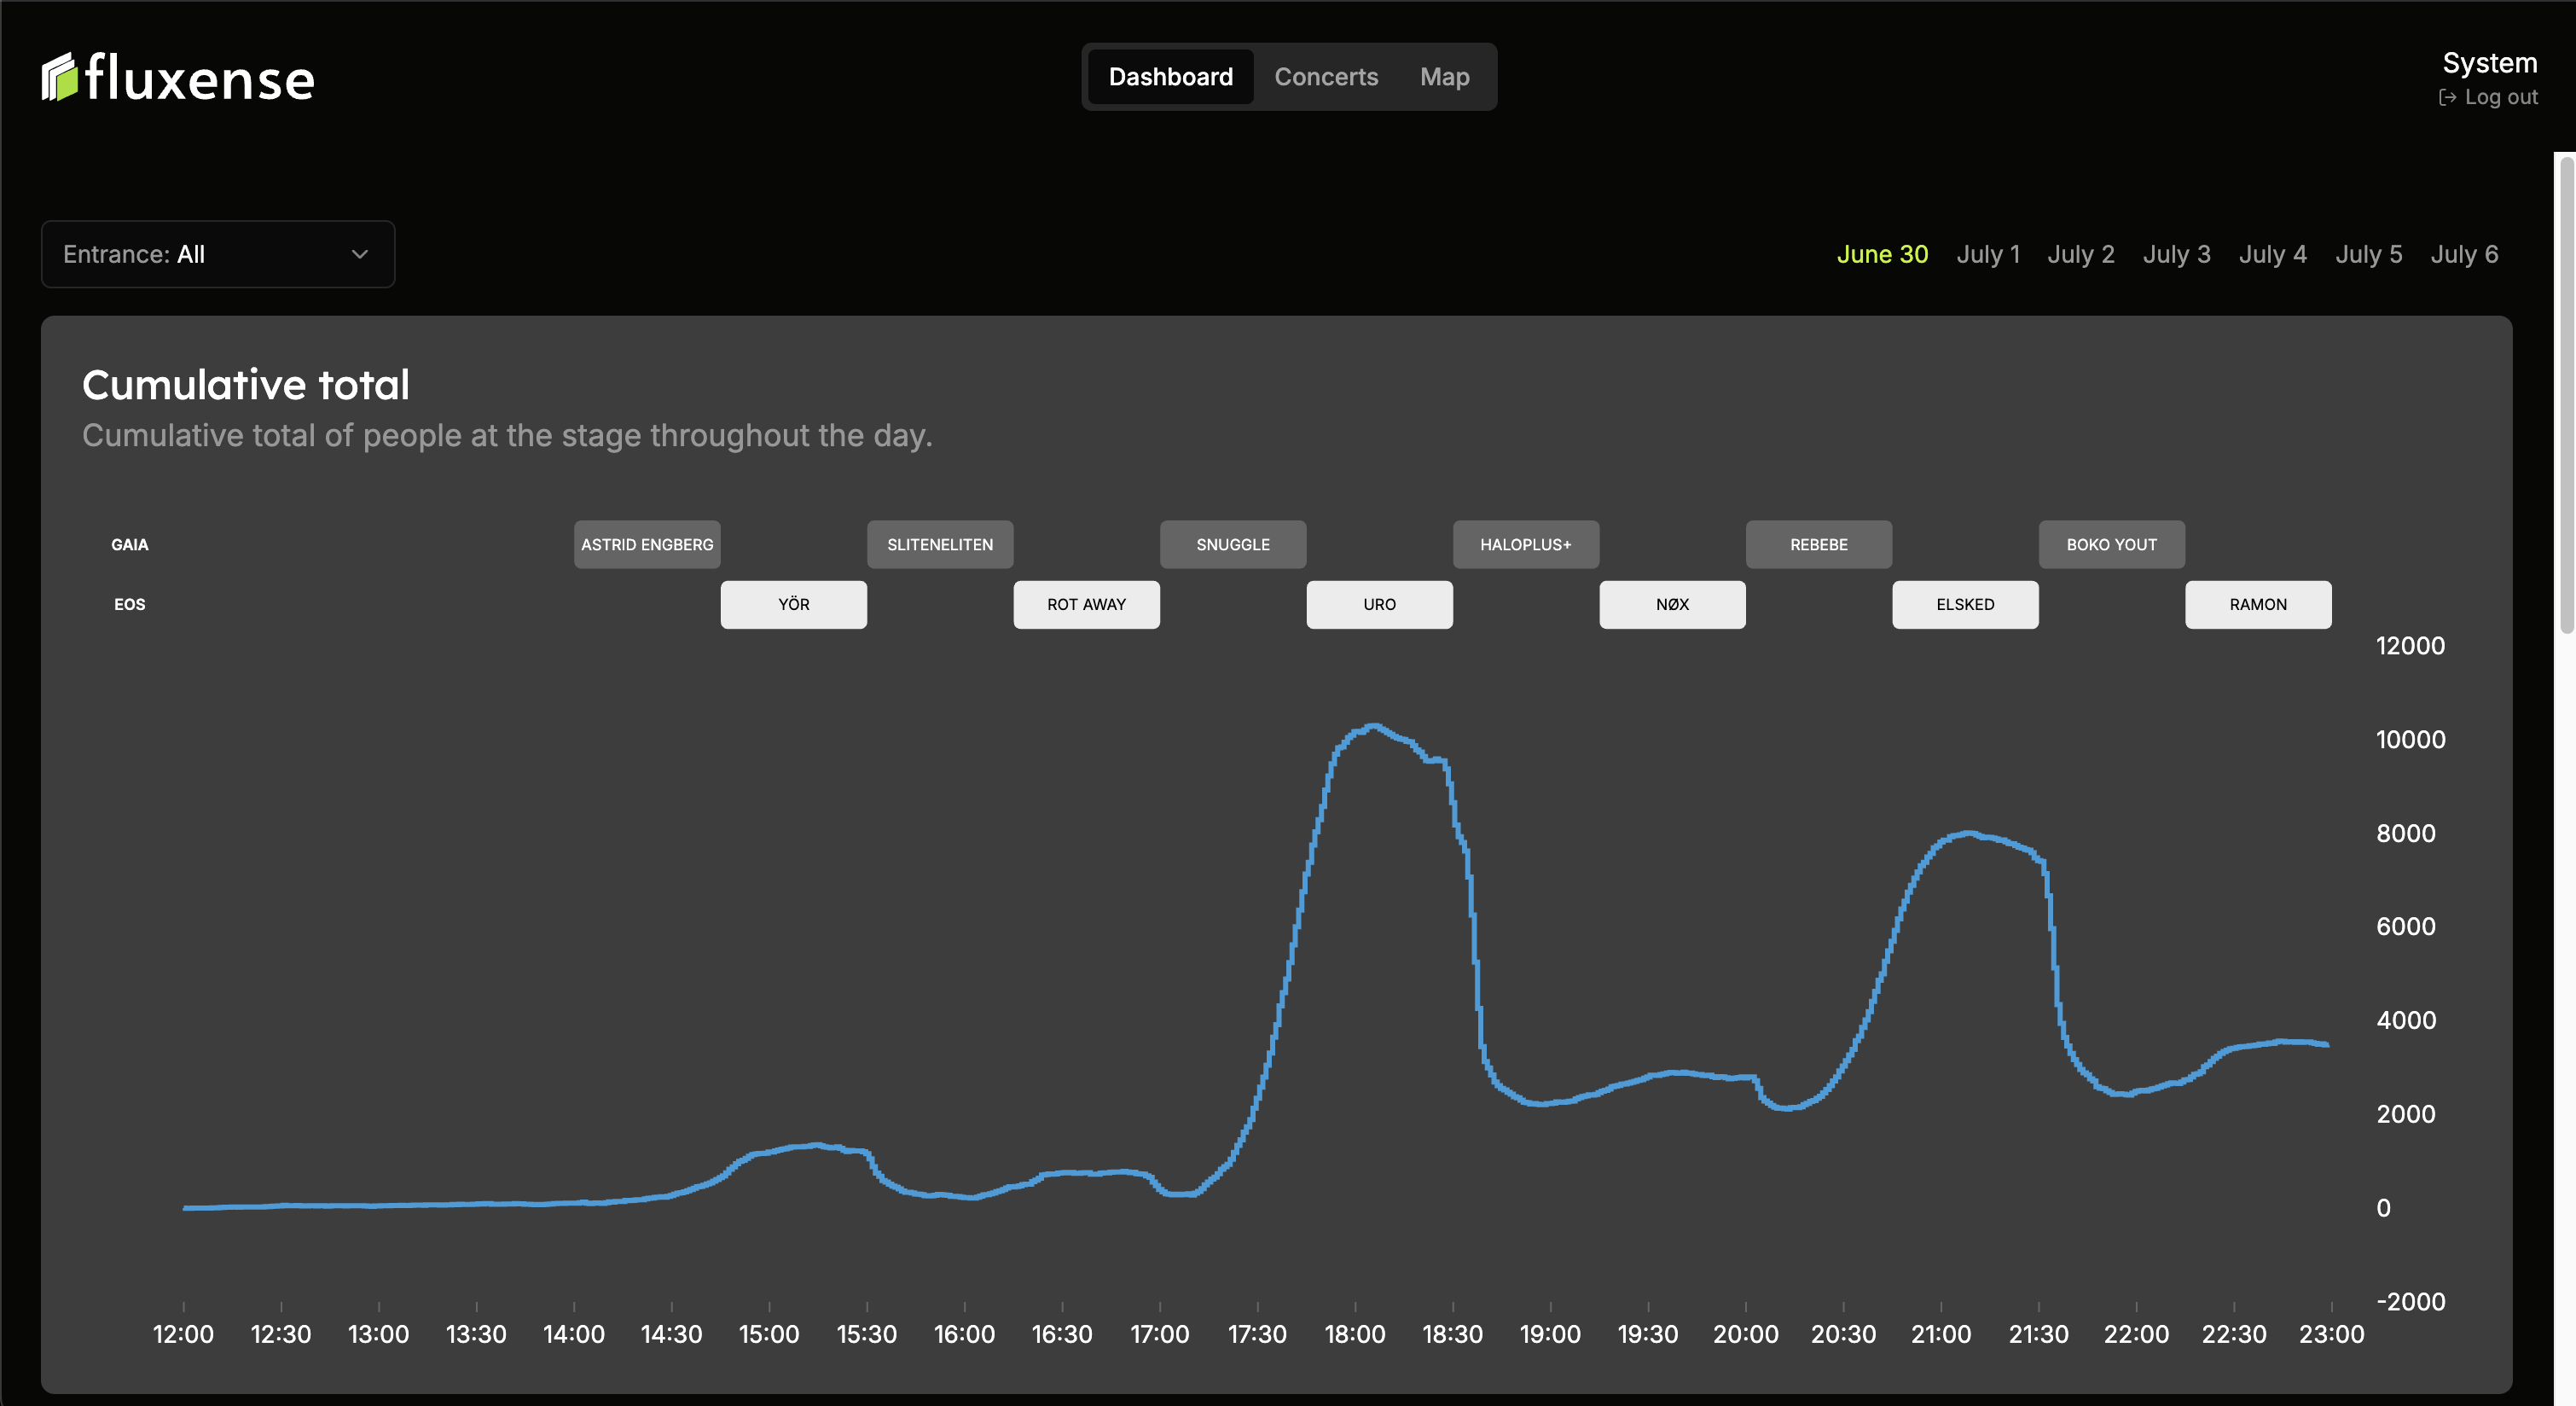
\includegraphics[width=\textwidth]{Pictures/Misc/Frontend/cum_total.png}
  \caption{The 'Dashboard' view displaying the cumulative total number of people estimated to be at the selected stage (Eos or Arena) throughout the day. An overlay along the top indicates the scheduled concert timings for the observed stage. Based on feedback requesting analysis of inter-stage flow (Appendix \ref{appendix:rf-sep-24}), schedules for adjacent stages (i.e., Gaia when observing Eos, or Orange stage when observing Arena) were also included.}
  \label{fig:showcase:dashboard}

\end{figure}


\begin{figure}[H]
  \centering
  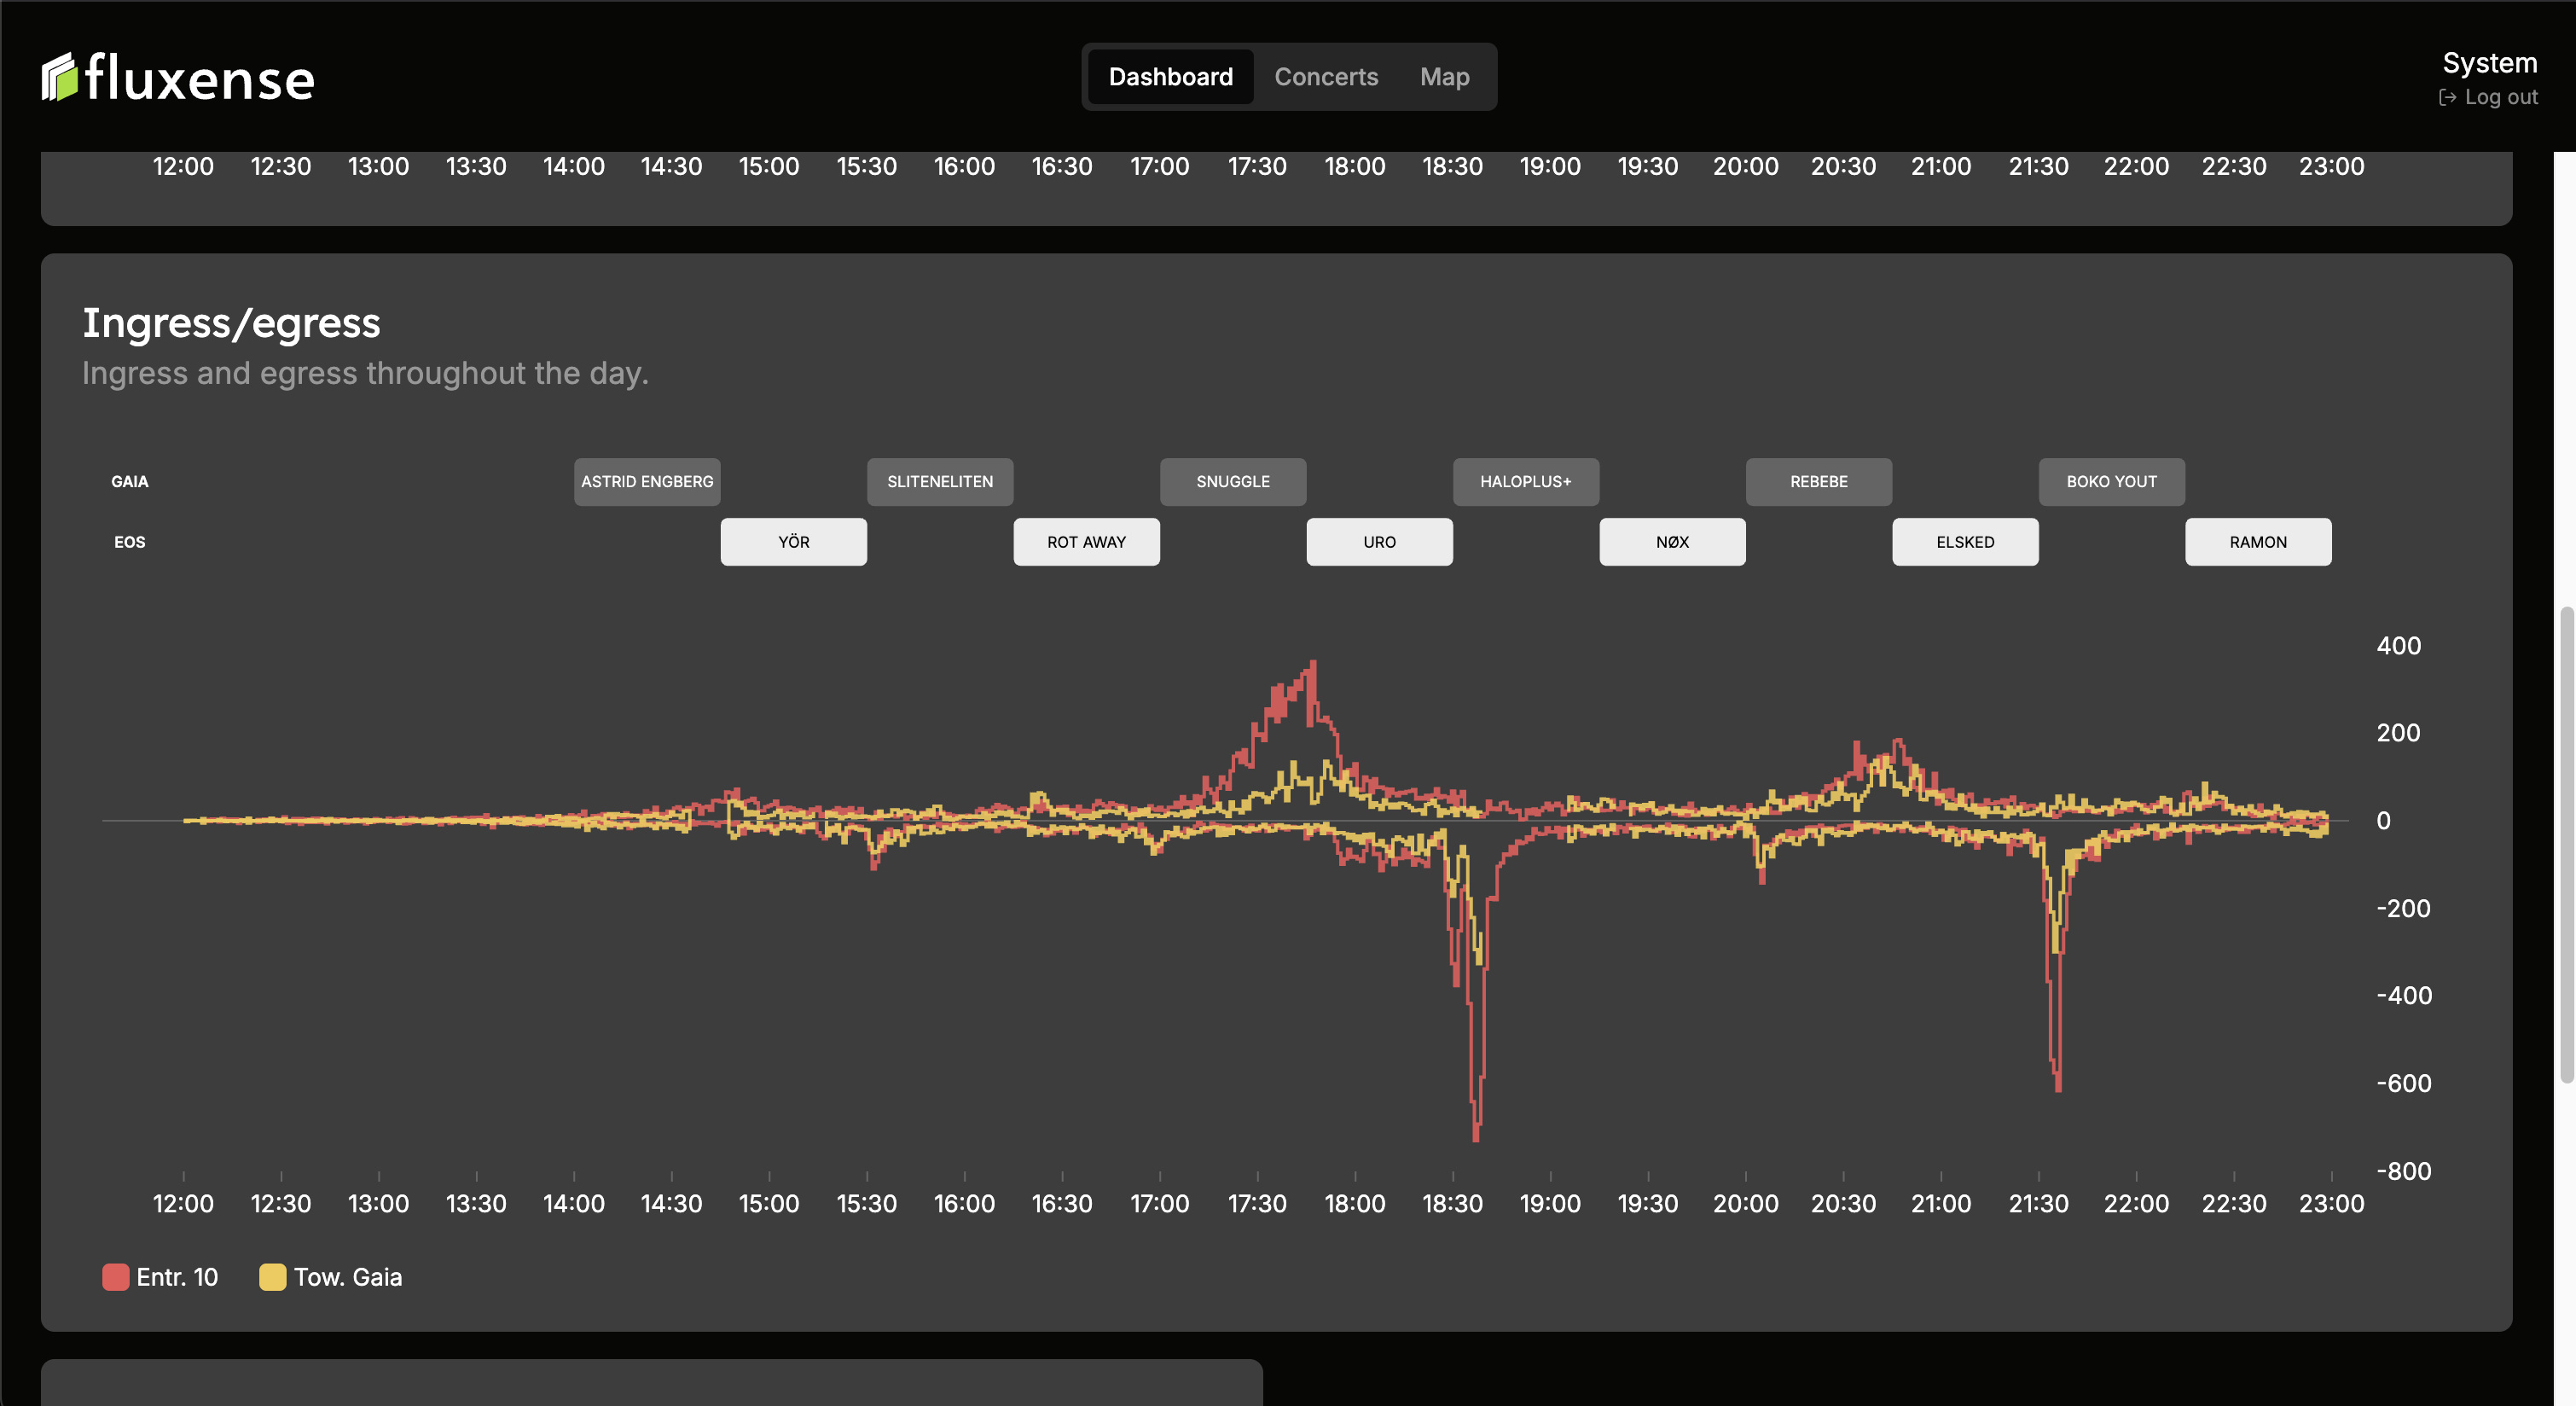
\includegraphics[width=\textwidth]{Pictures/Misc/Frontend/ingress_egress.png}
  \caption{The 'Dashboard' view showing the ingress (positive values) and egress (negative values) rates in people per minute throughout the day. Displaying data split by individual entrances (e.g., "Entr. 10", "Tow. Gaia") was implemented based on feedback requesting insight into the load of each entrance. The concert schedule overlay, including schedules from relevant adjacent stages added per user feedback, is also present for context.}
  \label{fig:showcase:ingress-egress}

\end{figure}


\begin{figure}[H]
  \centering
  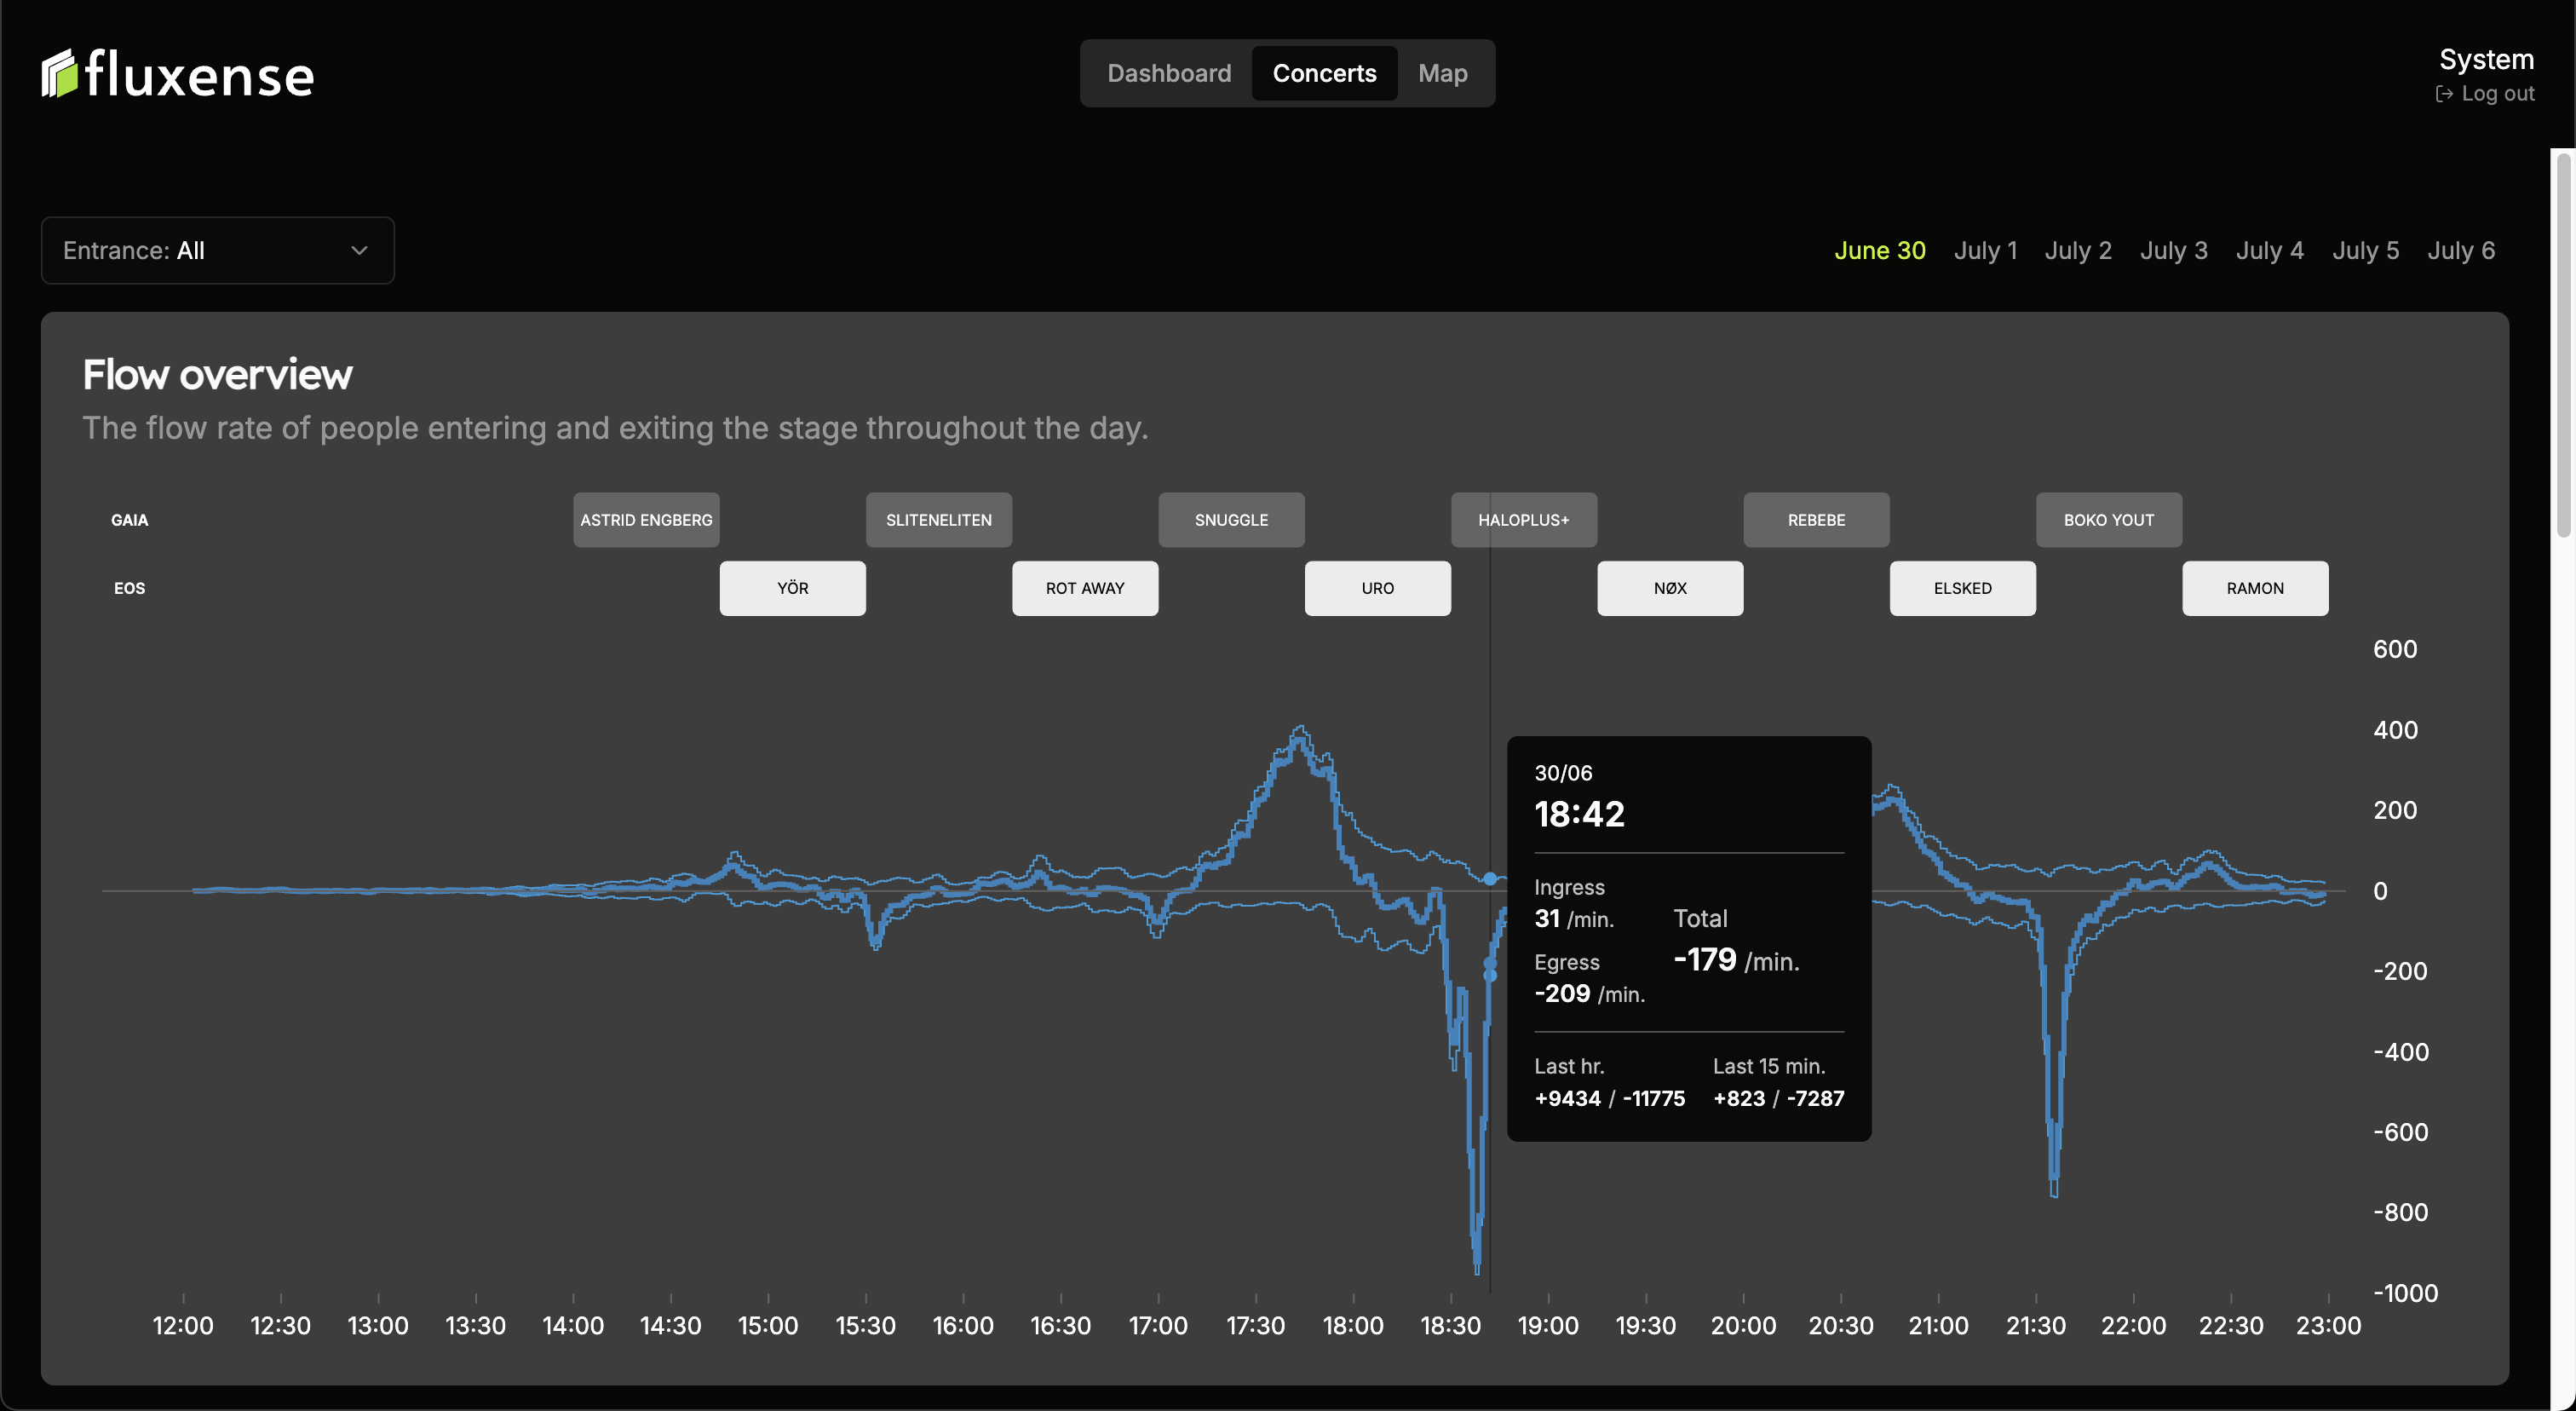
\includegraphics[width=\textwidth]{Pictures/Misc/Frontend/flow_total.png}
  \caption{The 'Concerts' view presenting the overall flow rates. It displays ingress-flow (top line), egress-flow (bottom line), and the total flow (bold middle line). Based on feedback, flow rates are presented in people per minute for easier interpretation compared to the initial people/second unit (Appendix \ref{appendix:rf-feb-25}). Hovering over the chart reveals a tooltip displaying instantaneous ingress, egress, and total flow rates at a given minute, along with aggregated ingress/egress totals over the last 15 and 60 minutes, aligning with RF's requested analysis intervals. The concert schedule overlay is also present for context.}
  \label{fig:showcase:flow-total}

\end{figure}

\begin{figure}[H]
  \centering
  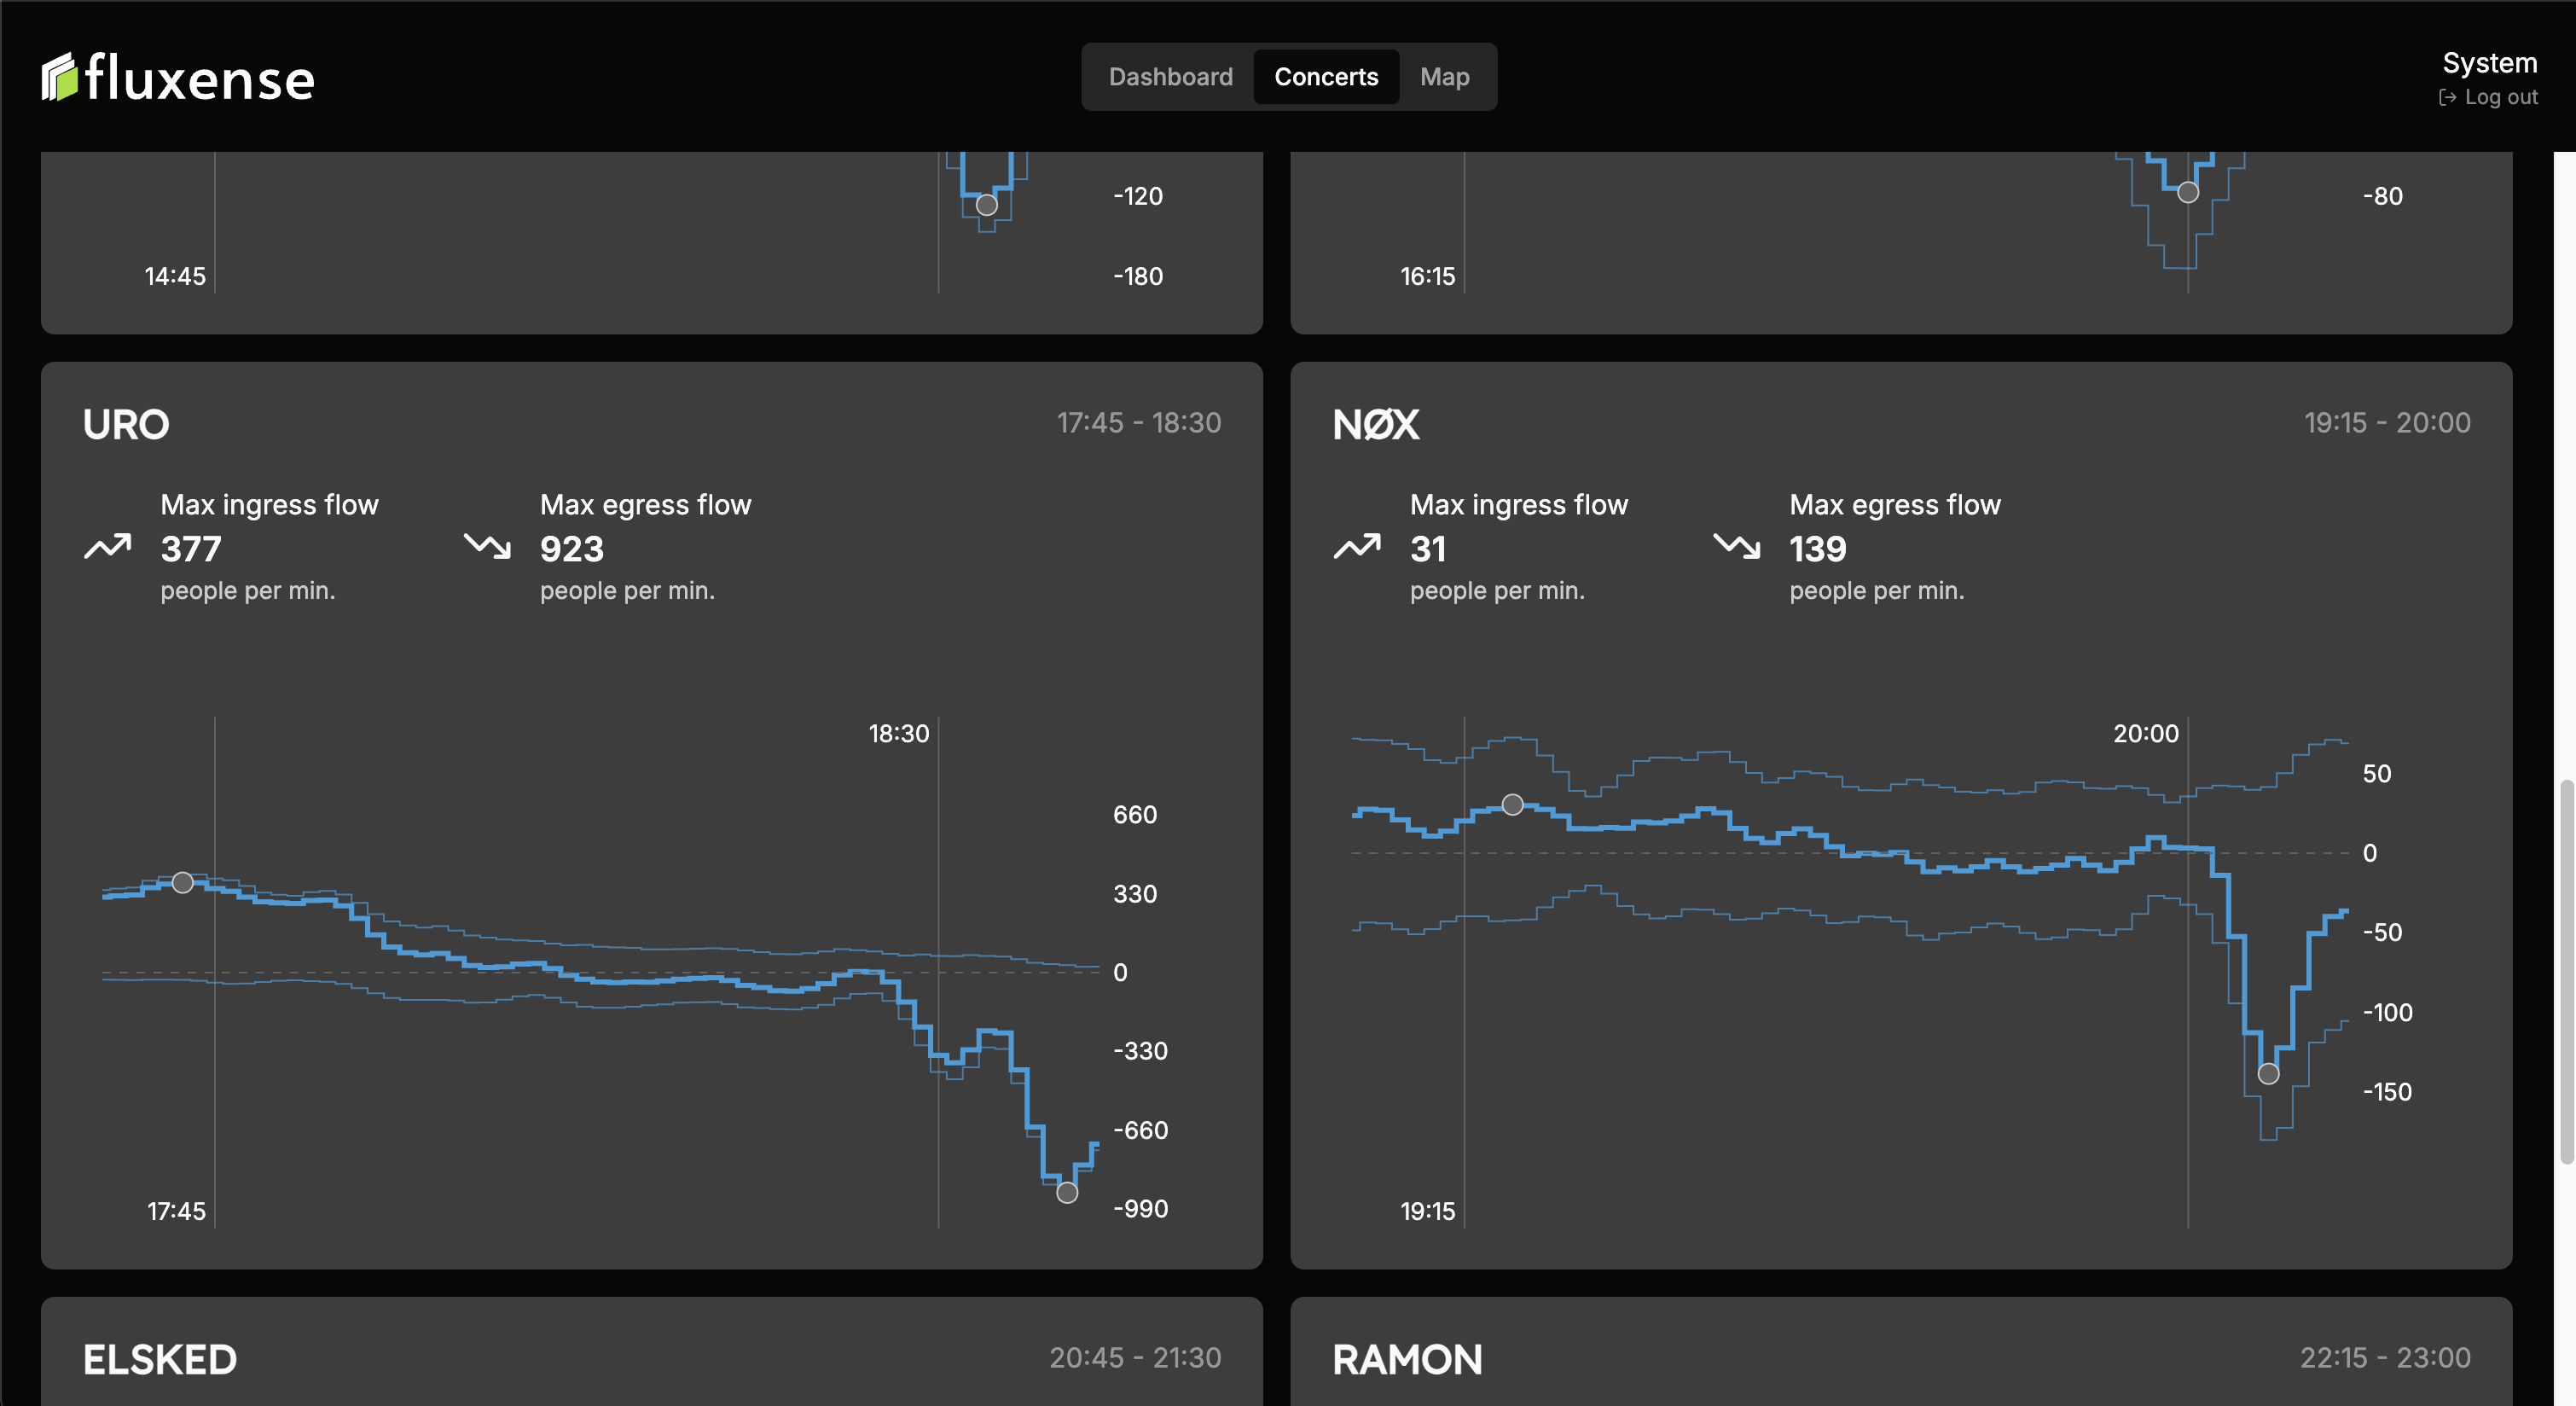
\includegraphics[width=\textwidth]{Pictures/Misc/Frontend/flow_concerts.png}
  \caption{The 'Concerts' view, with a breakdown of the flow rate data for individual concerts scheduled on the selected day. Each concert card shows the flow during the concert period and highlights the maximum observed ingress and egress flow rates in people per minute. The concert start/end times are also represented by vertical lines on the chart. This feature allows for analysis of flow rates relative to concert scheduling.}
  \label{fig:showcase:concerts}

\end{figure}

\begin{figure}[H]
  \centering
  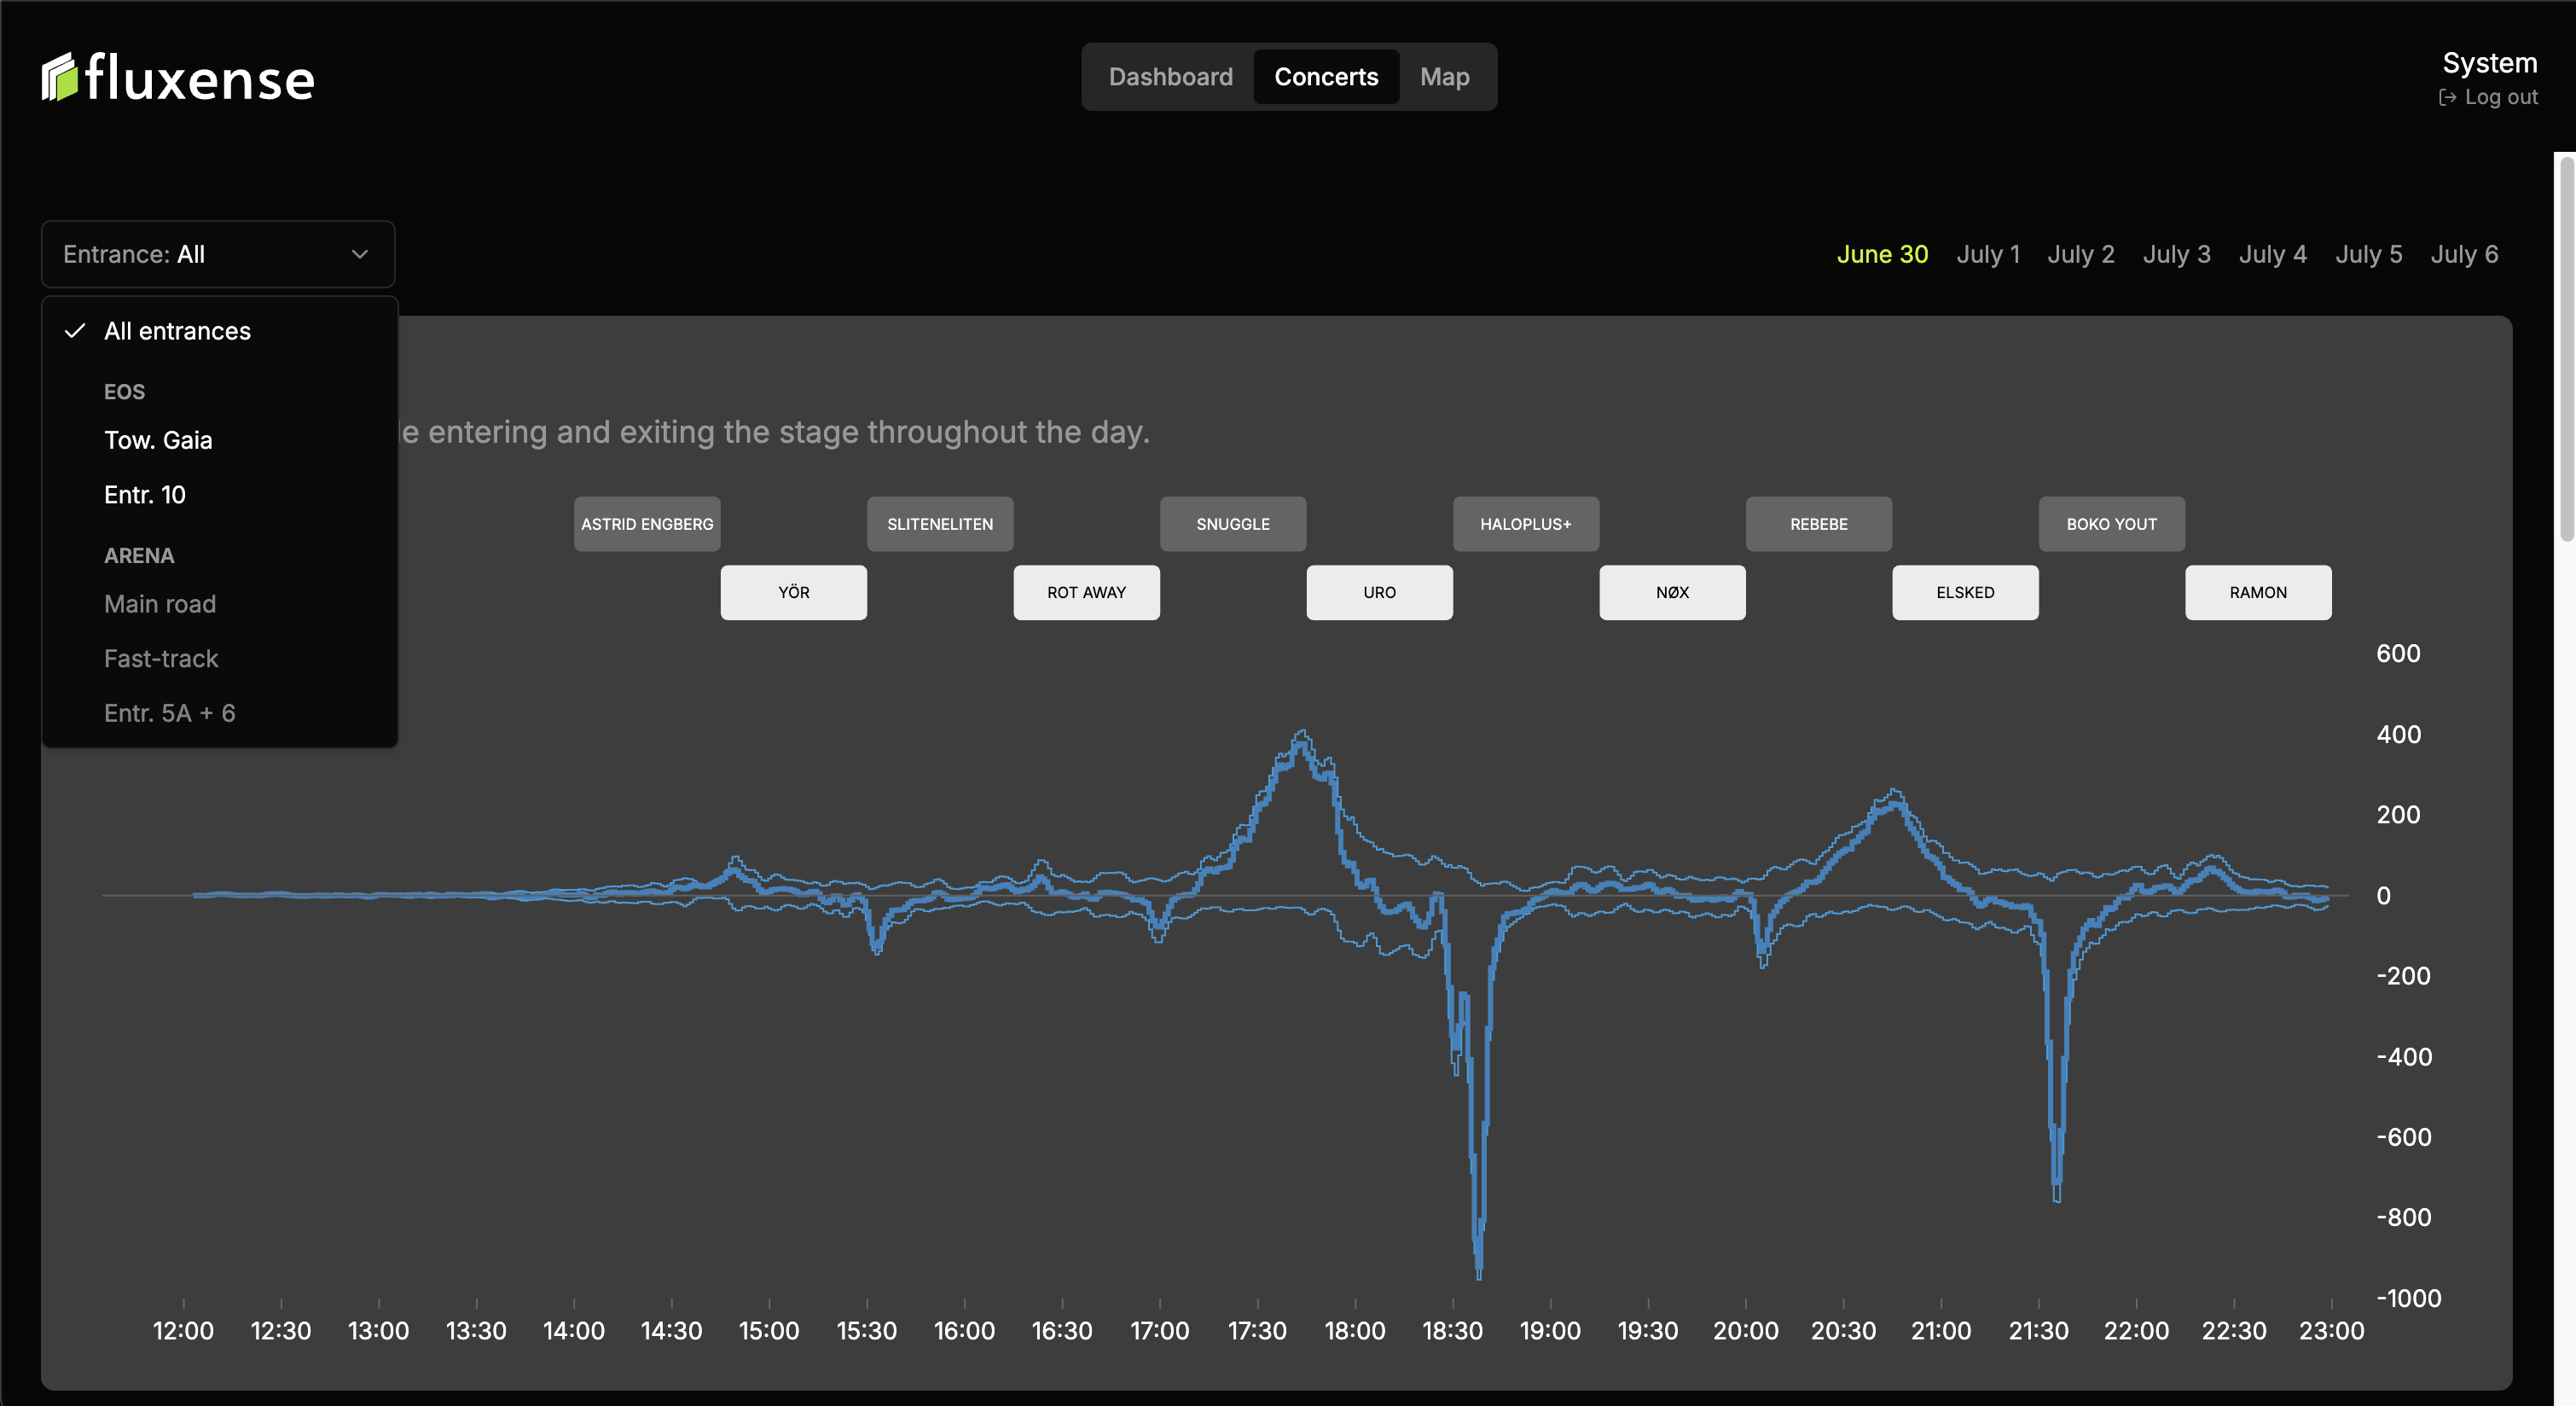
\includegraphics[width=\textwidth]{Pictures/Misc/Frontend/entrance_filter.png}
  \caption{The filtering controls available in the application, refined based on user requirements identified during feedback sessions. Users can select the date and filter the displayed data by specific entrances or view aggregated data for all entrances at a stage.}
  \label{fig:showcase:filter}
\end{figure}

\begin{figure}[H]
  \centering
  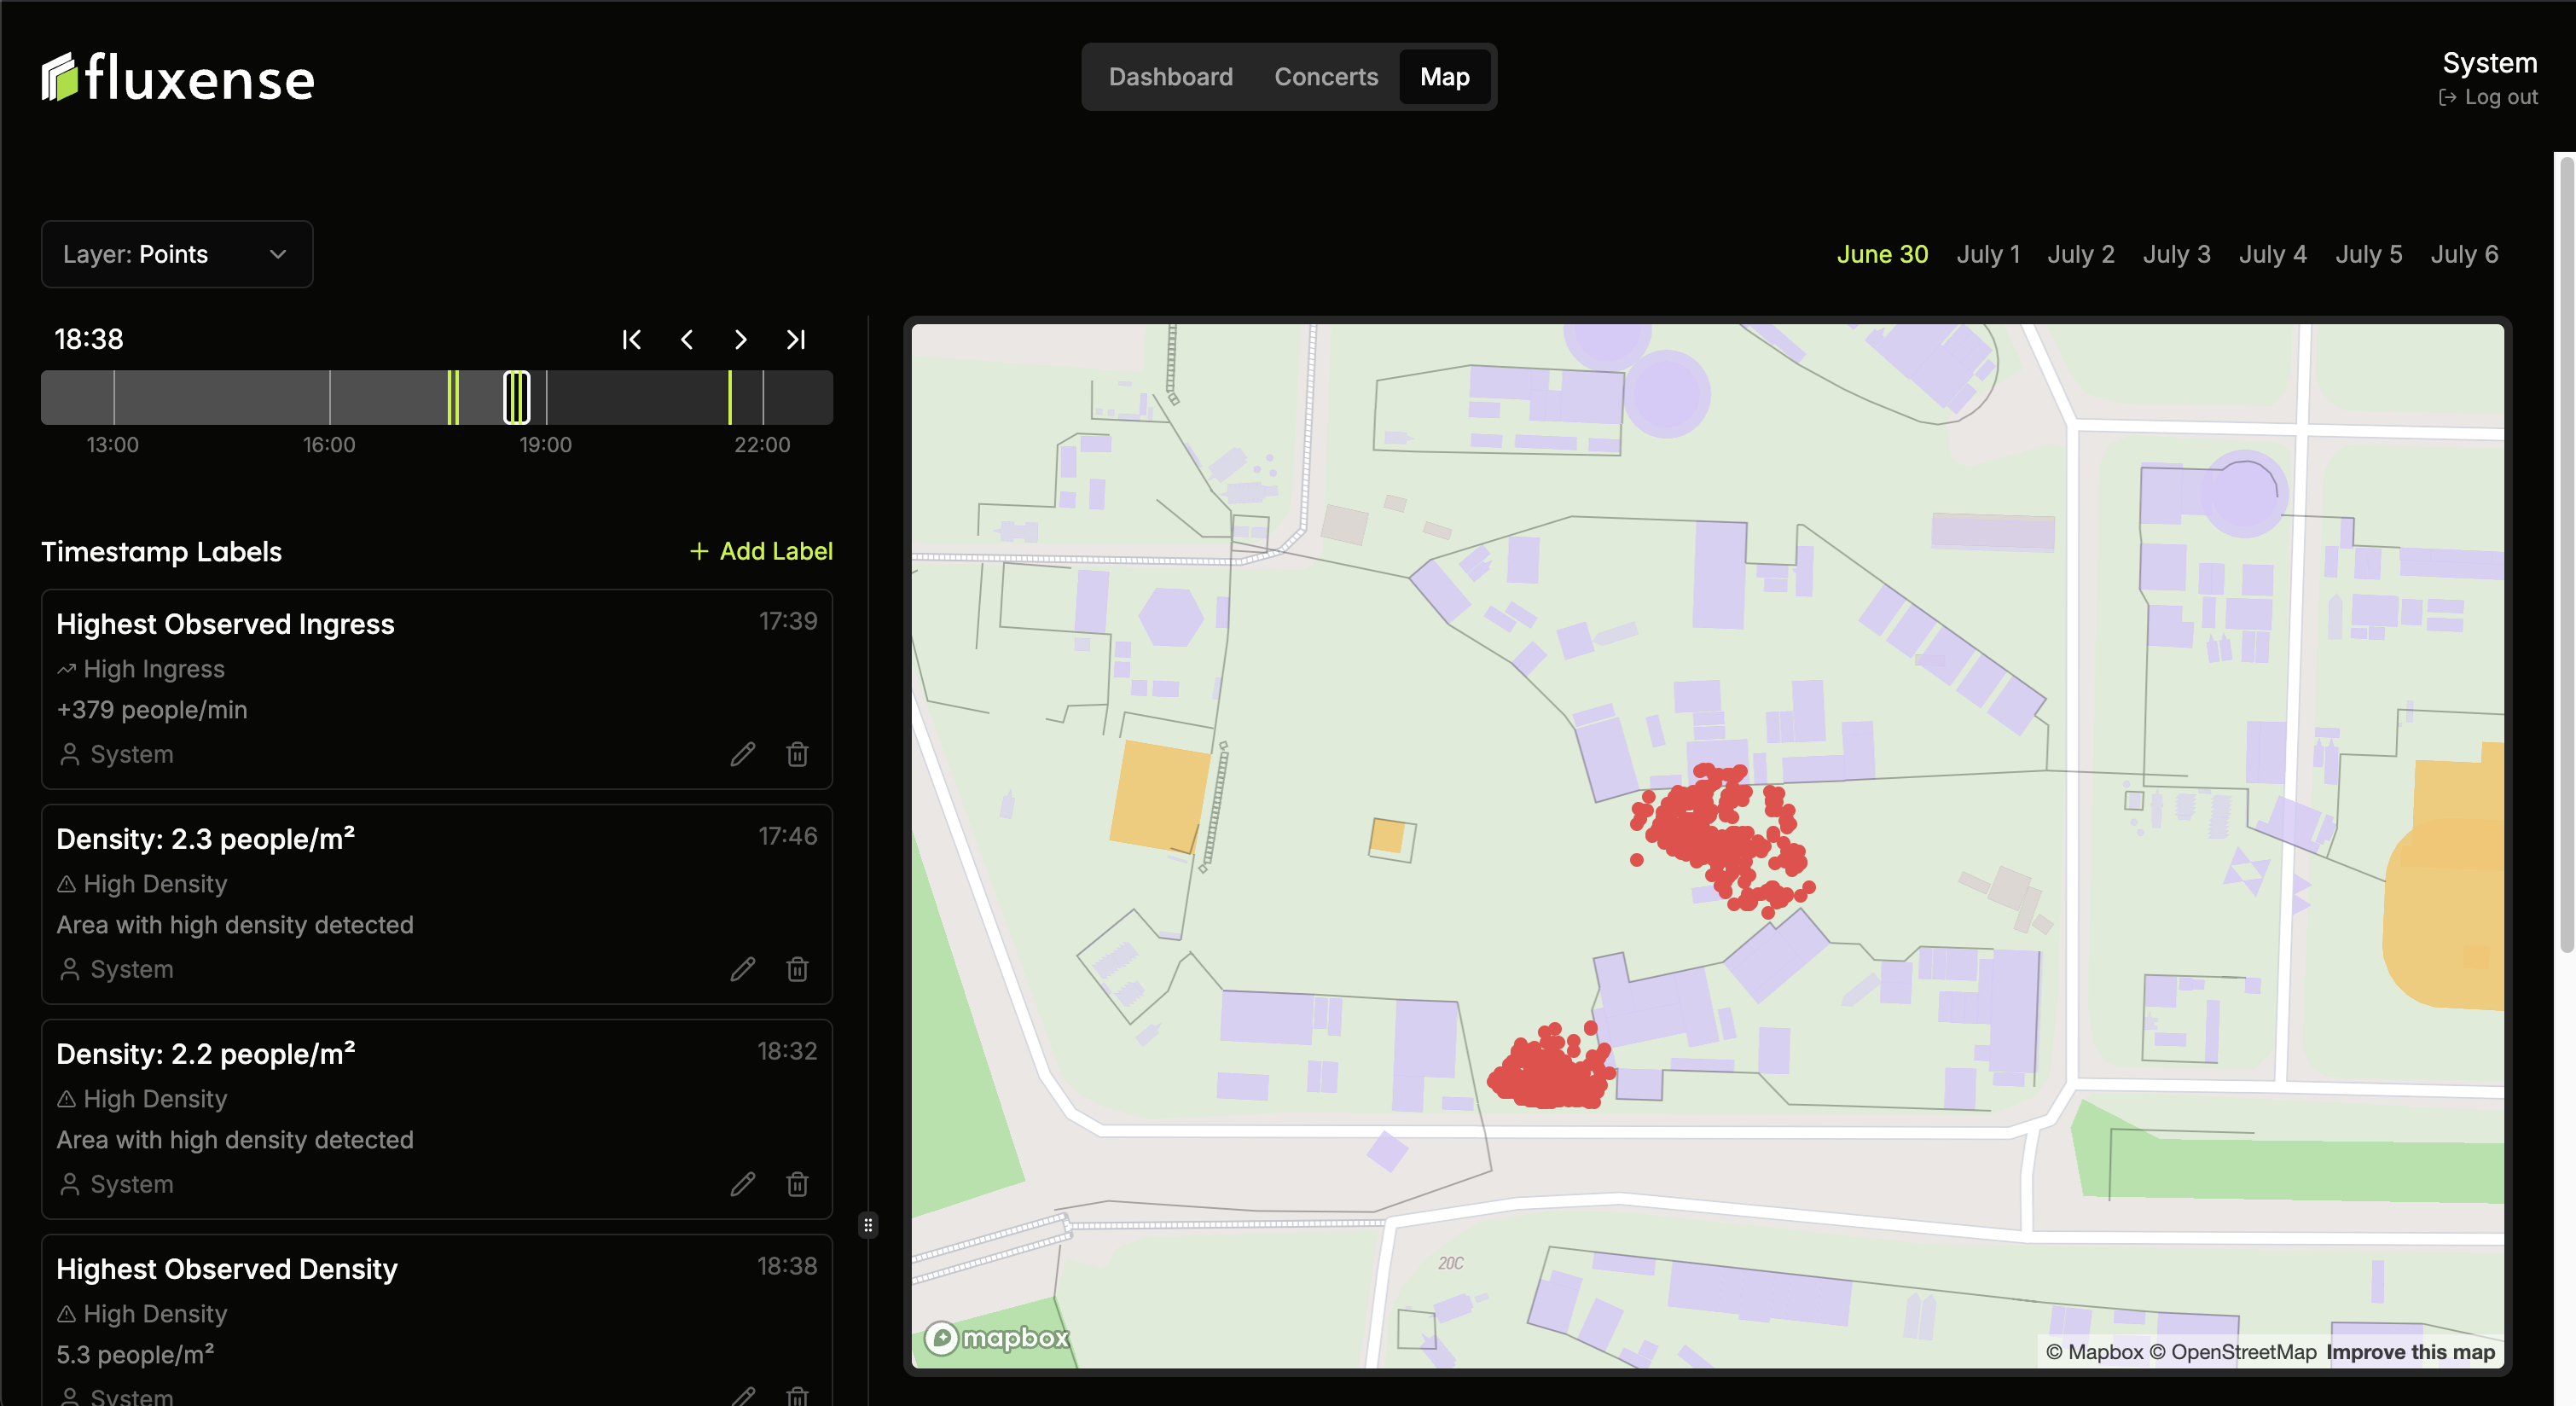
\includegraphics[width=\textwidth]{Pictures/Misc/Frontend/map_points.png}
  \caption{The 'Map' view interface elements. This includes an interactive timeline slider for navigating through the day, the 'Timestamp Labels' feature for adding notes, and the map displaying positional data for the selected time. The map layer itself can be configured to show individual detections as scatter points, as seen here.}
  \label{fig:showcase:map-scatter}

\end{figure}

\begin{figure}[H]
  \centering
  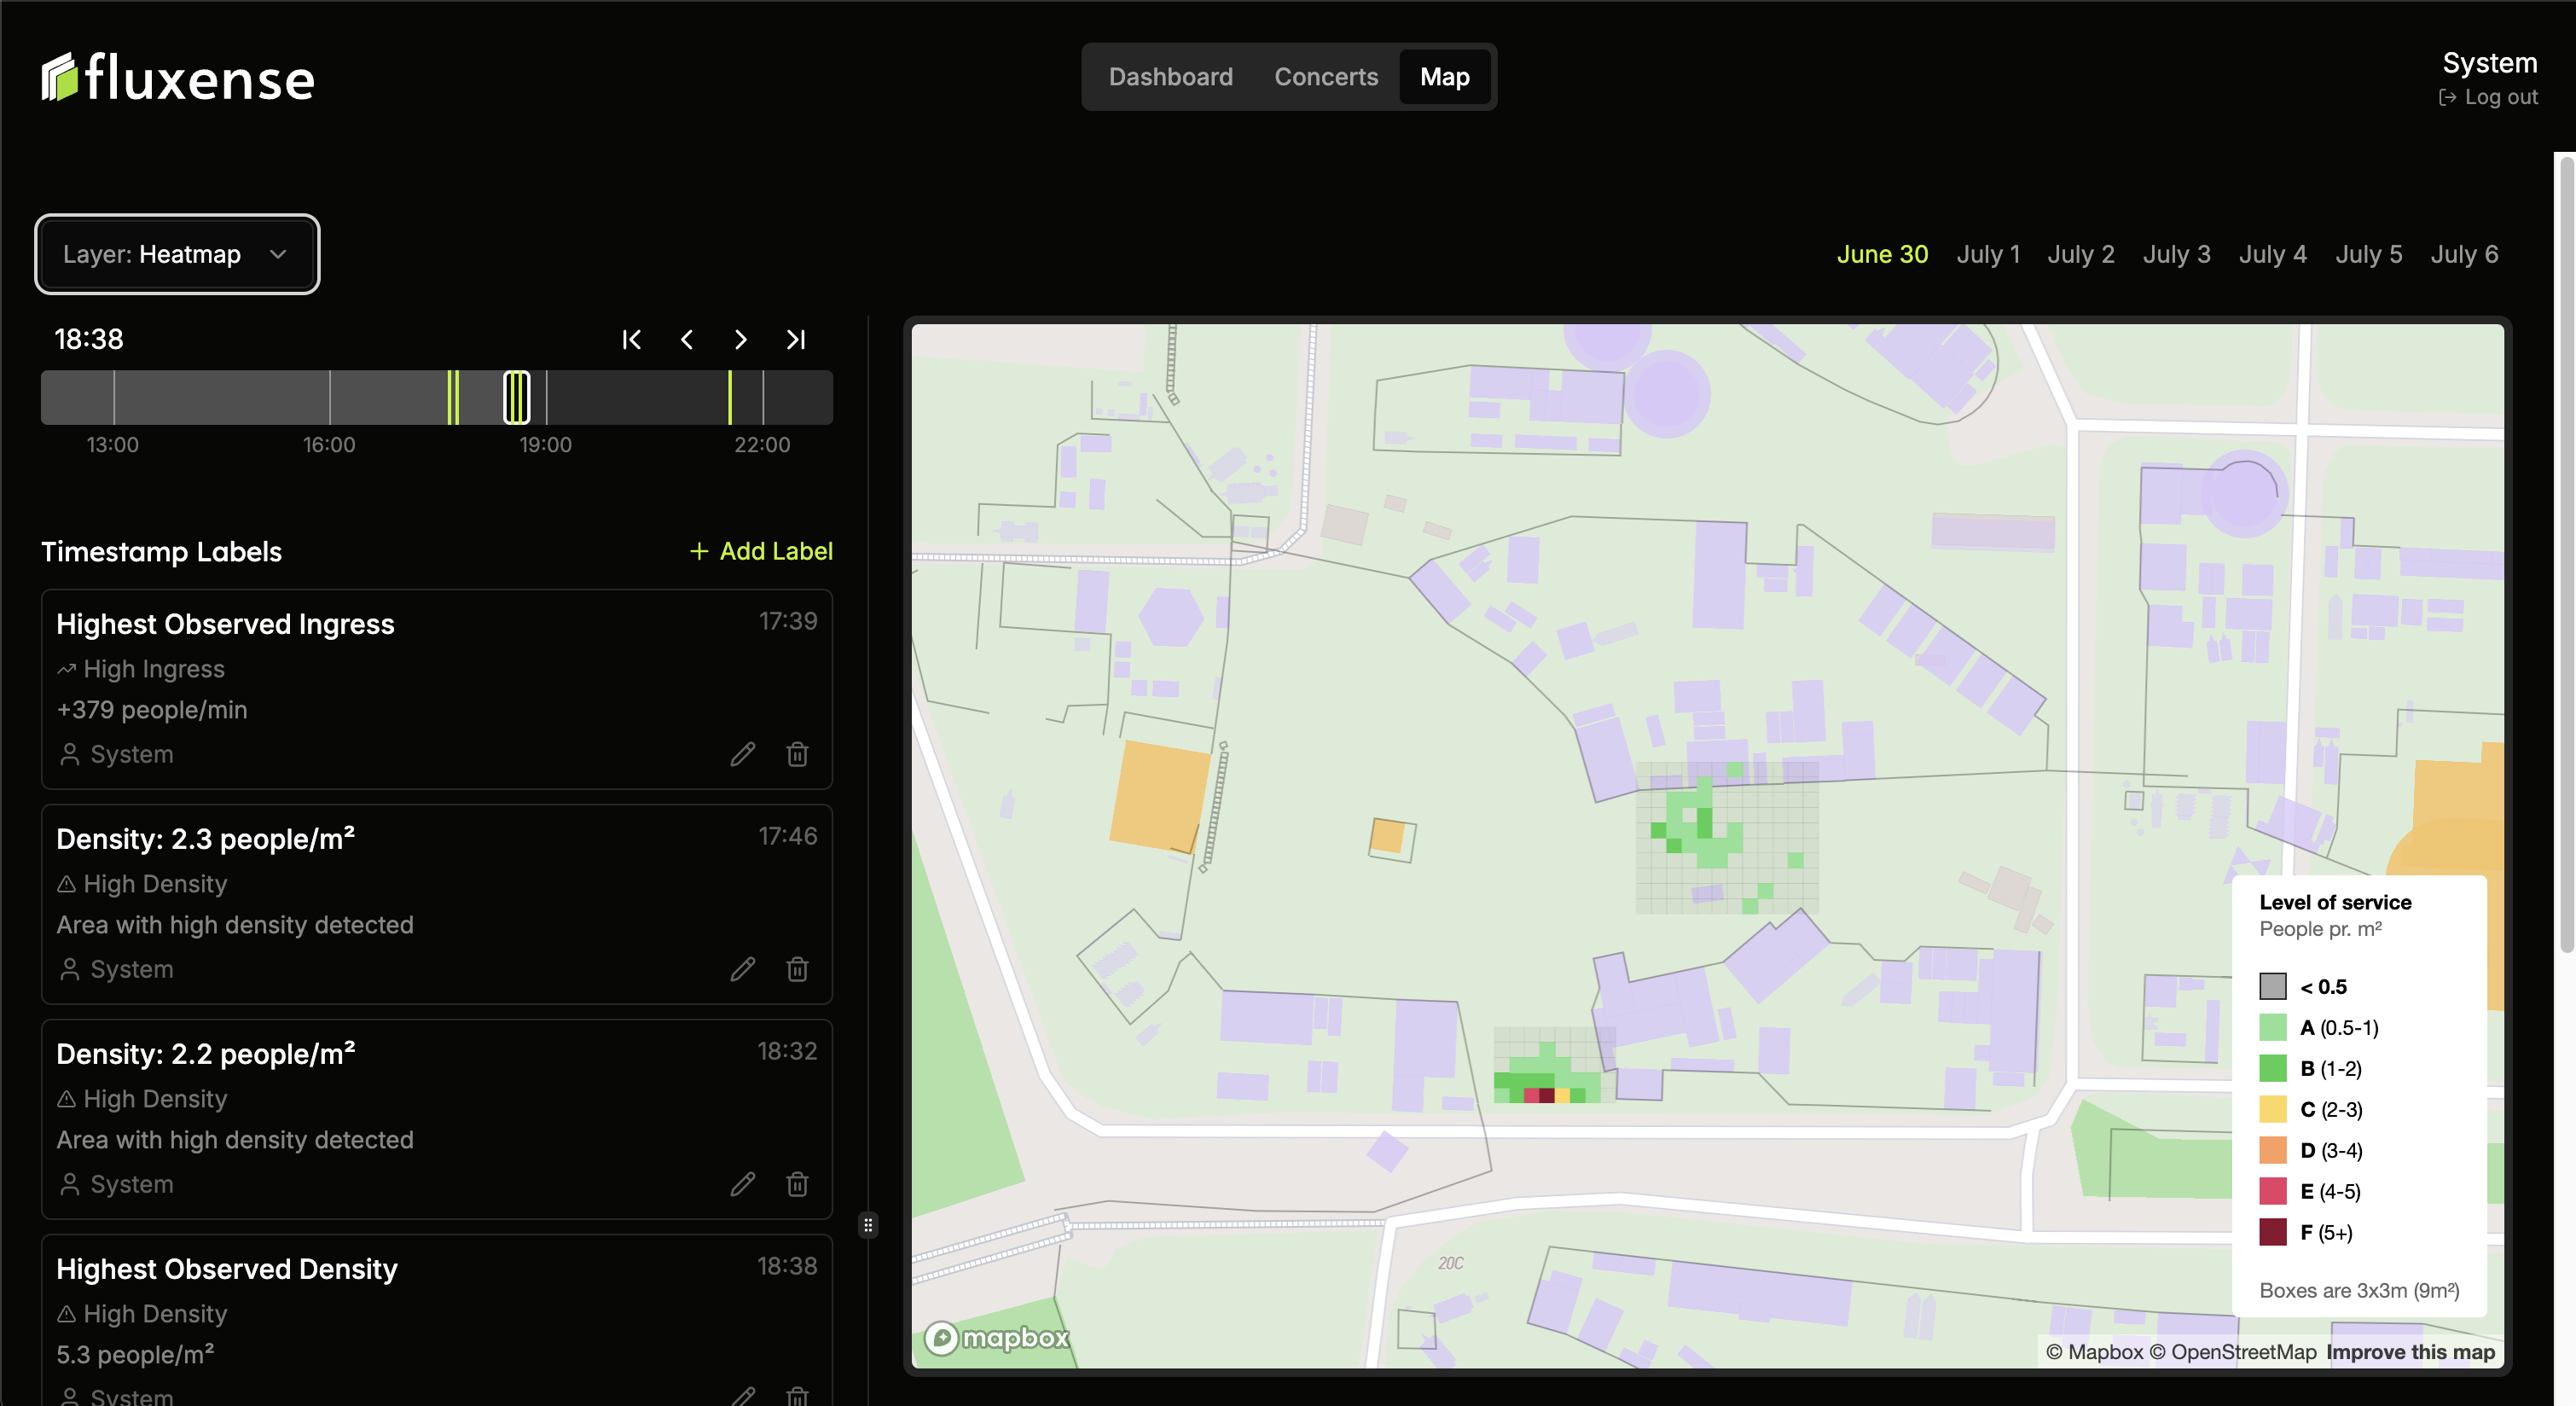
\includegraphics[width=\textwidth]{Pictures/Misc/Frontend/map_density.png}
  \caption{The 'Map' view displaying the 'Heatmap' layer. Crowd density is visualized using colored 3x3 meter grid cells. Following feedback, the color scale corresponds to Roskilde Festival's internal Levels of Service (LoS) scale (A-F), indicating people per square meter (people/m\textsuperscript{2}) to align with their existing practices.}
  \label{fig:showcase:map-density}

\end{figure}

\begin{figure}[H]
  \centering
  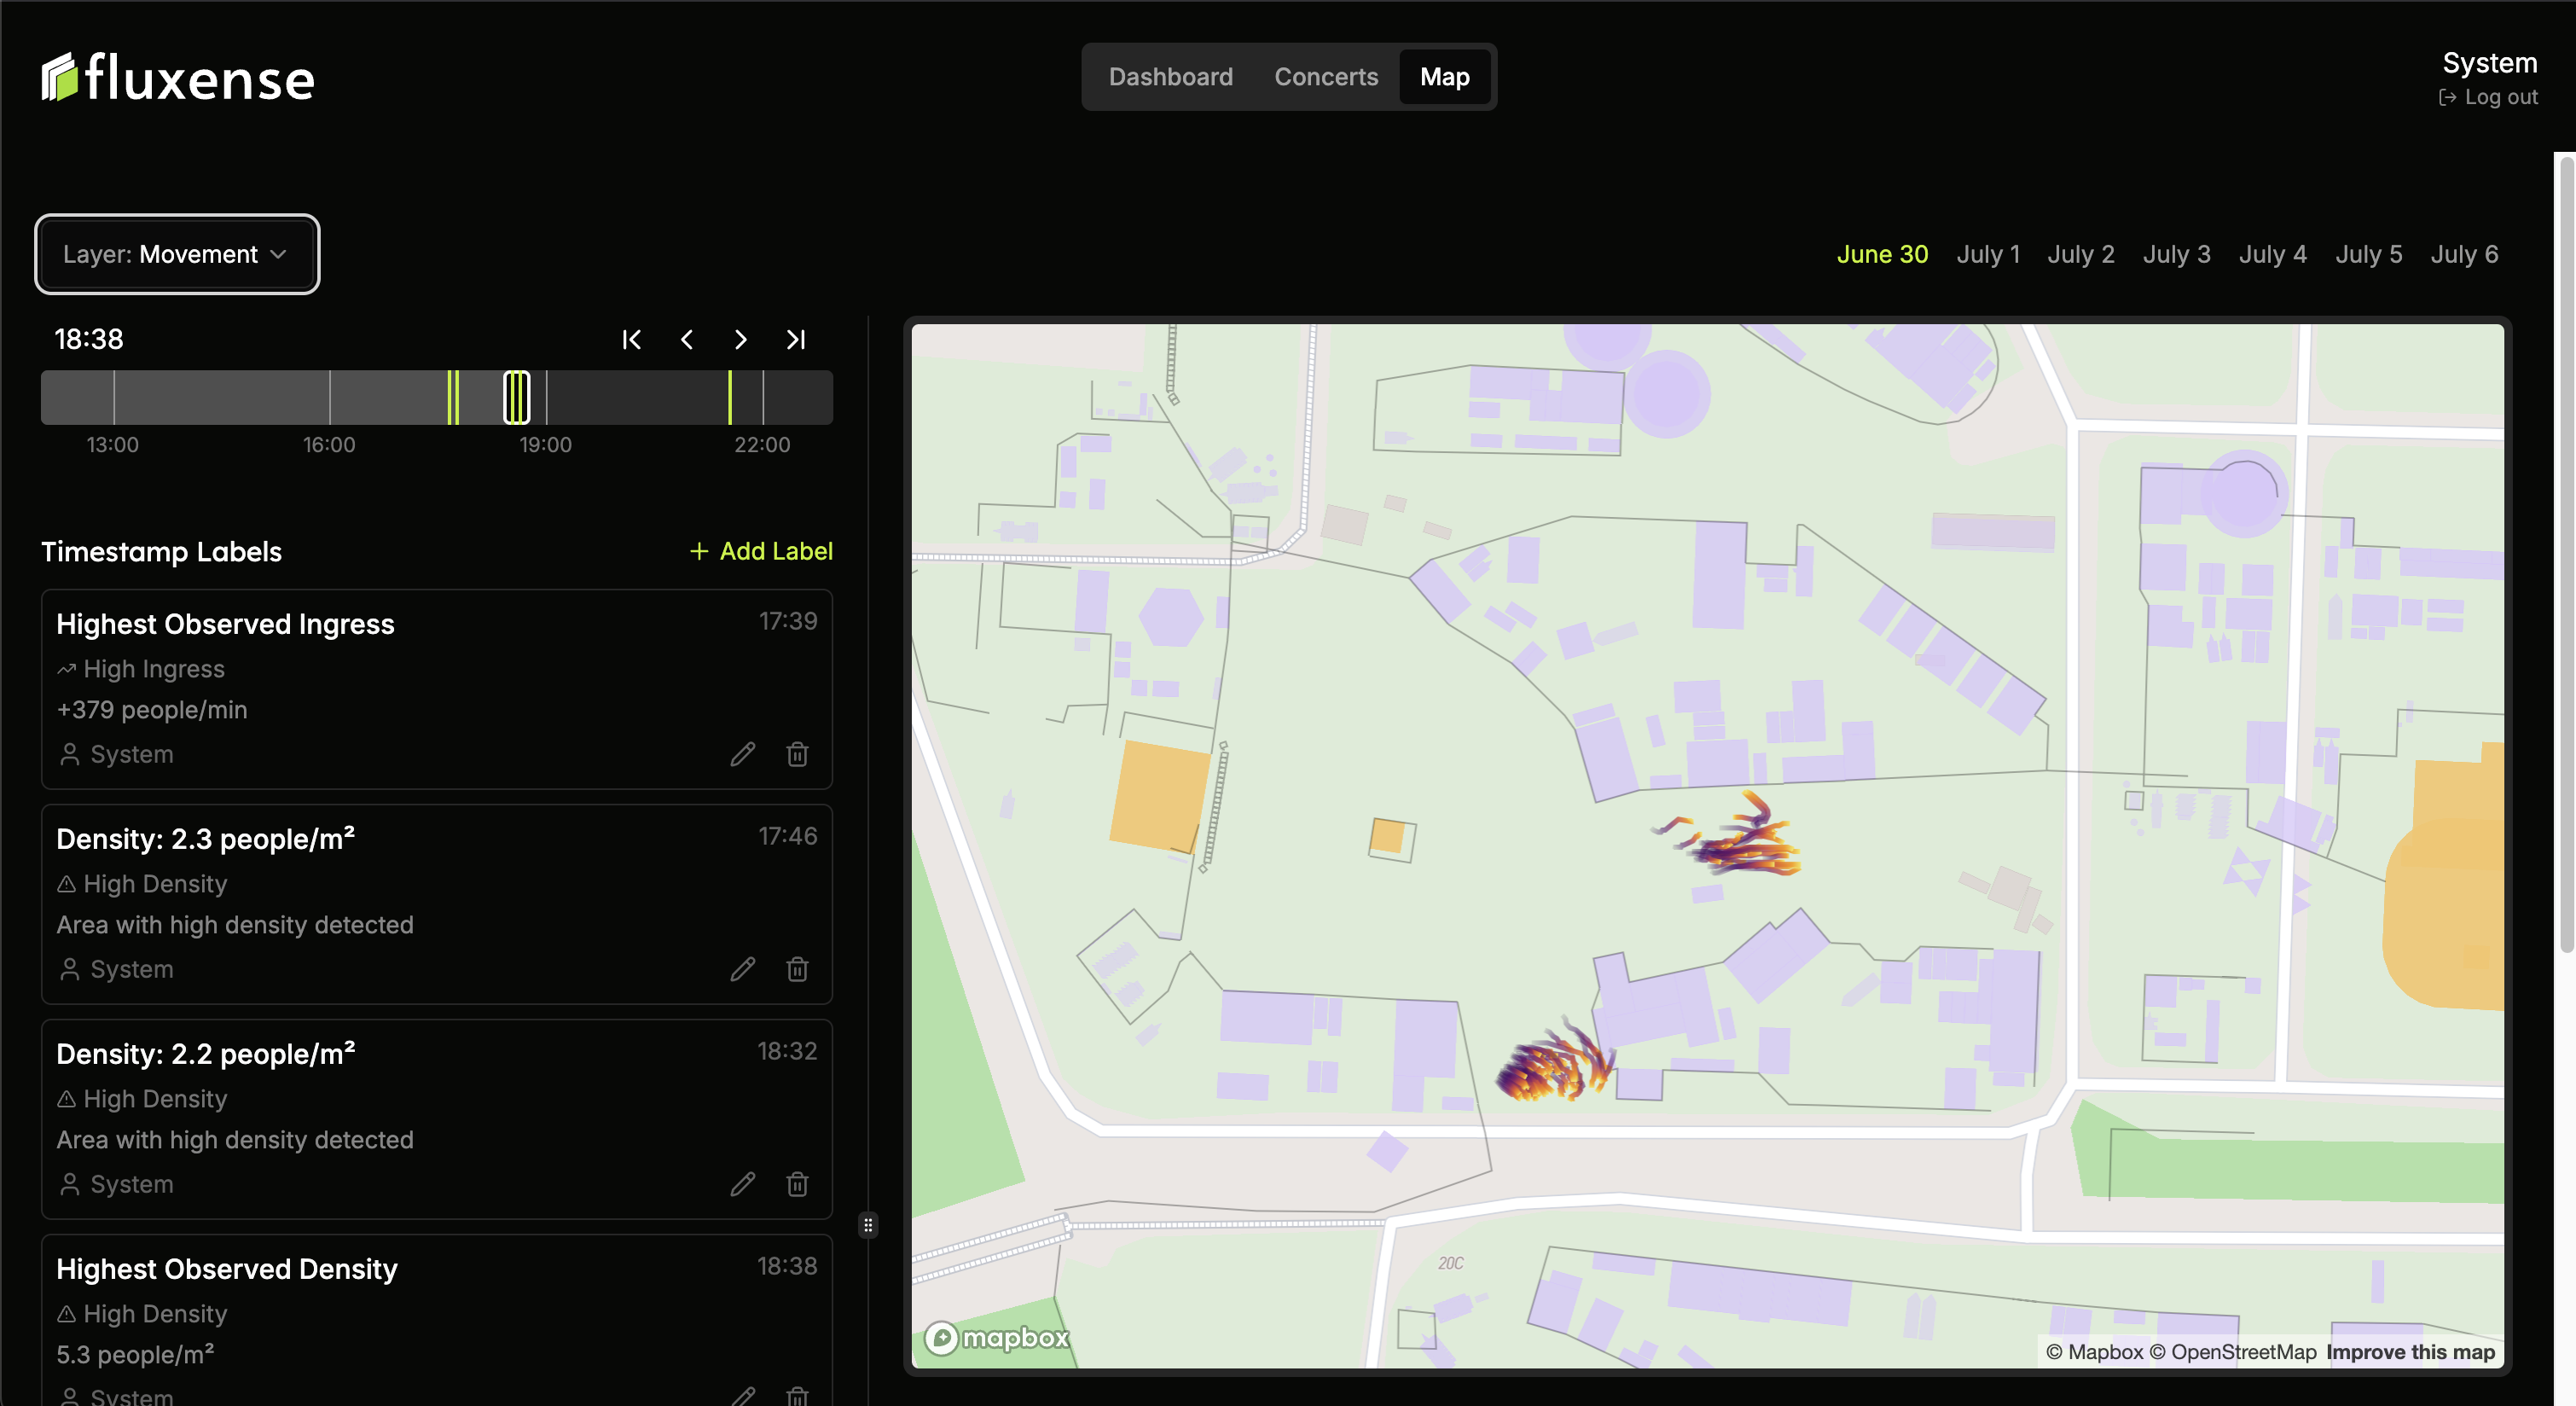
\includegraphics[width=\textwidth]{Pictures/Misc/Frontend/map_movement.png}
  \caption{The 'Map' view displaying the 'Movement' layer. Developed in response to feedback requesting visualization of movement patterns, it shows the trajectories of tracked individuals as lines on the map, with color gradients indicating the direction of movement (yellow being the latest position, and purple the initial position), helping to visualize flow and origin-destination patterns.}
  \label{fig:showcase:map-movement}

\end{figure}


\begin{figure}[H]
  \centering
  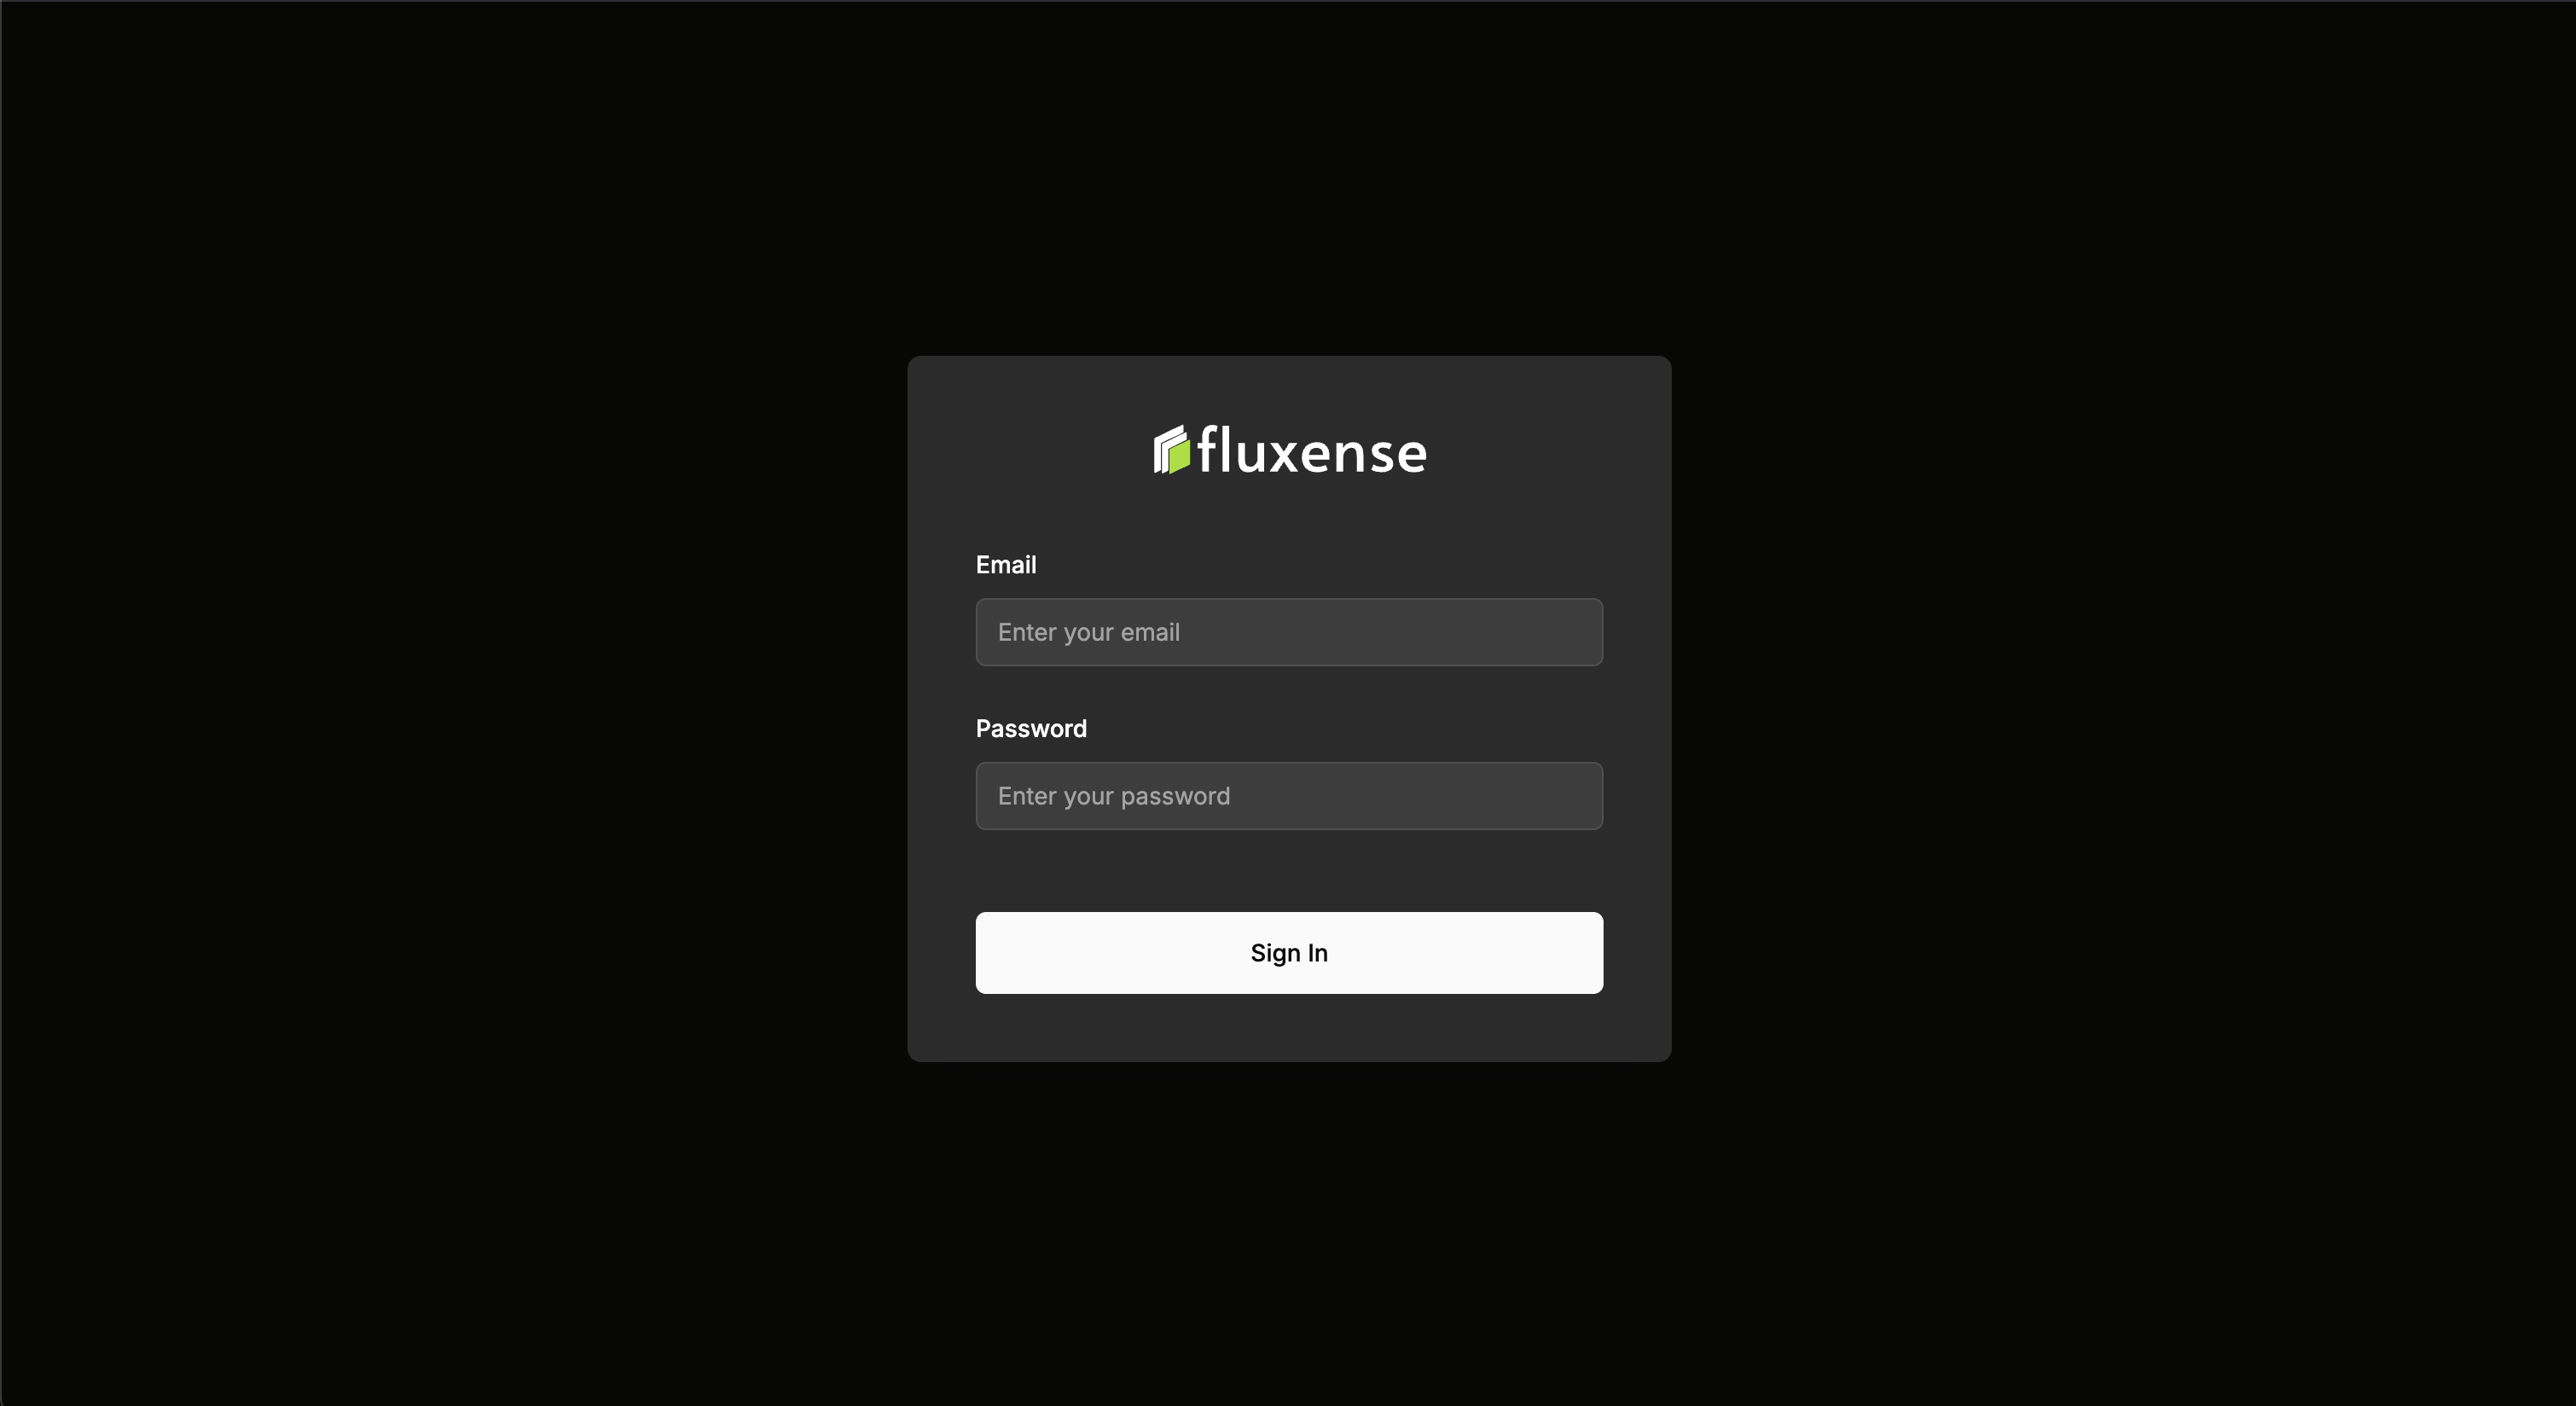
\includegraphics[width=\textwidth]{Pictures/Misc/Frontend/login.png}
  \caption{The application login screen, ensuring secure access to the crowd analysis data.}
  \label{fig:showcase:login}

\end{figure}

\section{Measure}
This section presents an evaluation of the technical performance of the developed product, as well as an assessment of the product with the Roskilde Festival safety team. The assessment was conducted through a workshop with key members of the safety team, where they were presented with the product and asked to provide feedback on its performance and value as compared to their existing workflows.


\subsection{Technical performance}
\label{sec:technical-performance}

The computer vision model selected for detecting individuals in video footage was YOLOv8, which was subsequently fine-tuned for the specific task of head detection (Section \ref{sec:cv_model}). This fine-tuned model is further referred to as \textit{yolo\_heads}. The rationale for selecting YOLOv8 included its balance of high inference speed and robust detection accuracy, making it suitable for processing extensive video data efficiently (as noted in Section \ref{sec:cv_model}). To optimize performance for the unique conditions of each camera's viewpoint and the general festival environment, separate \textit{yolo\_heads} models were trained using custom annotated frames extracted from video recordings from each specific camera deployment at the Eos and Arena stages.

The performance of the \textit{yolo\_heads} models was evaluated using standard object detection metrics: Precision, Recall, and F1-score. Precision measures the accuracy of the positive predictions (i.e., what proportion of detected heads were actual heads). Recall measures the model's ability to find all actual heads (i.e., what proportion of actual heads in the frames were detected). The F1-score provides a harmonic mean of Precision and Recall, offering a single measure of the model's accuracy. It thus symmetrically represents both precision and recall in one metric. As is standard in evaluation of machine learning models, a separate test set of annotations was used to evaluate the model's performance. This ensures that the performance assessment is not biased by the data used for training the model. \newpage

Precision, Recall, and F1-score are defined as follows:

\begin{center}
  \centering
  $\text{Recall} = \frac{\text{TP}}{\text{TP} + \text{FN}}, \qquad
    \qquad  \text{Precision} = \frac{\text{TP}}{\text{TP} + \text{FP}}, \qquad
    \qquad  \text{F1-score} = 2\cdot \frac{\text{precision} \cdot \text{recall}}{\text{precision} + \text{recall}}$
\end{center}

where TP (True Positives) is the number of correctly predicted heads, FP (False Positives) is the number of incorrectly predicted heads, and FN (False Negatives) is the number of heads that were not detected by the model.

The results for the \textit{yolo\_heads} models on footage from Arena's \textit{CAM1}, \textit{CAM2}, and \textit{CAM2}, as well as Eos' \textit{CAM2} and \textit{CAM4} are presented in Table \ref{tab:yolo_performance}. Note that \textit{CAM1} and \textit{CAM3} at Eos stage were not utilized, as they were redundant to \textit{CAM4} and \textit{CAM1} respectively. \textit{CAM4} at Arena stage was also not utilized due to time constraints.

The high precision demonstrates that the model is fairly accurate in its predictions, with a low number of false positives. In other words, when the model predicts a head, it is correct 87\% of the time on average. The recall is lower however, indicating that the model captures around 71\%, or misses 29\%, of heads captured by the camera. This essentially means that there are rarely \textit{fewer} people in the frame than the model detects. \textit{CAM1} at Arena stage brings the recall average down significantly, likely due to the camera's tall position, leading to smaller, harder to discern heads in the frame. More training data could help improve these results, as the model was only trained on a limited number of frames, mostly due to time constraints of the project.

\begin{table}
  \centering
  \renewcommand{\arraystretch}{1.15}
  \begin{tabularx}{0.9\textwidth}{@{} ll >{\centering\arraybackslash}X >{\centering\arraybackslash}X >{\centering\arraybackslash}X @{}}
    \toprule
    Stage                                   & Camera         & Precision (\%) & Recall (\%)    & F1-Score (\%) \\
    \midrule
    \multirow{2}{*}{Eos}                    & CAM2           & 91.23          & 76.52          & 83.23         \\
                                            & CAM4           & 86.94          & 81.84          & 84.32         \\
    \midrule
    \multirow{3}{*}{Arena}                  & CAM1           & 79.92          & 41.25          & 54.42         \\
                                            & CAM2           & 92.62          & 84.01          & 88.11         \\
                                            & CAM3           & 84.62          & 70.97          & 77.19         \\
    \midrule \midrule
    \multicolumn{2}{@{}l}{\textbf{Average}} & \textbf{87.07} & \textbf{70.92} & \textbf{77.45}                 \\
    \bottomrule
  \end{tabularx}
  \caption{Performance metrics of the fine-tuned YOLOv8 head detection model across different camera deployments at Roskilde Festival.}
  \label{tab:yolo_performance}
  \renewcommand{\arraystretch}{1.0}
\end{table}

% TODO: homography evaluation, cumulative total cumulative error, other metrics don't have intrinsic error



\subsection{Roskilde Festival workshop}
\label{sec:business-value}

In order to evaluate the business value of the developed product, a workshop was held with two key members of the Roskilde Festival safety team, Mads Therkilden (Safety Lead) and Niels Laustsen (Program Safety Team Lead). The workshop began with a demonstration of the results of the project, where participants were shown the final product and its capabilities, subsequently providing login credentials to access the application themselves. The remainder was structured around a series of scenarios that the safety team might encounter during the planning of the festival. The scenarios were designed in order to test whether the developed product could provide a concrete value in situations related to the hypotheses in Section \ref{sec:problem-definition}. The scenarios were as follows:

\begin{enumerate}
  \item \textbf{Scenario 1:} Entrance 10 is a primary access point for the Eos stage, especially crucial during the first days. Let's assume festival-goer feedback from Roskilde Festival (RF) 2024 suggested this entrance felt congested at times. The safety team needs to assess if the current width is adequate or requires modification for RF 2025 to handle peak demand safely.
  \item \textbf{Scenario 2:} Your colleague from Food \& Beverage (F\&B) proposes moving the popular Cava Bar to the main corridor leading to/from Entrance 10 to capture more foot traffic. The safety team is concerned because they believe this corridor already experiences some congestion during peak times. Adding a bar with likely queues could create unsafe scenarios. The task is to explain to the F\&B colleague these concerns and justify recommending against the relocation.
  \item \textbf{Scenario 3:} A colleague questions the back-to-back scheduling of the Eos and Gaia stages during the first days, concerned that it could lead to congestion between the stages. How can you determine and communicate whether or not the scheduling strategy was operationally sound?
\end{enumerate}

After presenting each scenario, the participants were requested to discuss how they would approach the scenario given their current workflows. Once they reached an agreement, they were asked to use the application to aid in solving the same scenario. After each the scenario, the participants were presented with a series of questions, aimed at quantitatively evaluating the business value of the product. The results of this evaluation can be found in (Appendix \ref{appendix:workshop-evaluation}). The questions were as follows:

\begin{enumerate}
  \item Overall, compared to your current process, how valuable do you perceive the approach using this tool to be for this specific task? (\textit{Scale 1-5: Not at all Valuable to Extremely Valuable})
  \item How do you think using this tool might impact the time or effort required for this task compared to your current methods? (\textit{Scale 1-5: Much More Effort to Much Less Effort})
  \item Compared to your current process, how might using the tool affect your confidence in the outcome related to this task? (\textit{Scale 1-5: Much Less Confident to Much More Confident})
\end{enumerate}

These questions were designed to assess the perceived value of the product across several aspects. Effort reduction corresponds to potential monetary savings, but also allows for allocating time to other important planning tasks. Confidence enhancement should at the very least be neutral. Considering potential skepticism towards AI tools, a negative response would indicate that the product is not perceived as accurate enough for usage. Additionally, the participants were asked to rate their overall perception of the product's value for a given scenario, as well as provide any additional comments or feedback.

Assessing an issue such as in the first scenario, assessing Entrance 10, is challenging in the safety team's current workflows, as it heavily depends on the availability of relevant CCTV footage, which is not guaranteed. Assuming footage exists, the team would need to manually search through it, and make subjective density estimates based on the Levels of Service model presented in Figure \ref{fig:fruin}. Given access to the application, the team could immediately find the historical density data for the specific entrance, identify the peak moments (e.g., a brief 5.3 people/m\textsuperscript{2} spike), and observe a dissipation after only a few minutes. This aided the team in concluding that the short-lived peak was not concerning enough to warrant a significant change in the existing infrastructure.

The second scenario, concerning the Cava Bar relocation, clearly contrasted current communication efforts. Assuming the team has access to the information gathered in the first scenario, the current workflow relies heavily on verbal arguments to justify safety concerns to other departments, such as Food \& Beverage. If further justification is needed, Mads Therkildsen explained he would manually create visuals, for instance using PowerPoint, to illustrate theoretical concerns like cross-flow or queue formation -- a time-consuming process requiring skills outside their core competencies. Given the application, the team could instantly collect objective visual evidence by taking screenshots of density heatmaps or movement flow patterns.

Finally, the third scenario, involved back-to-back concert scheduling between Eos and Gaia. The current workflow bases planning on estimations: calculating required pathway widths using the theoretical maximum capacity of a stage (e.g., 8000 for Eos) and applying standard formulas based on pathway width. This method relies on assumptions about crowd size, which is currently impossible to accurately calculate, as well as expected behavior based on concert assessments, as discussed in Section \ref{sec:existing-frameworks}. The safety team subsequently used the application to identify actual peak attendance (closer to 10,000) and, more importantly, the actual peak flow rate through the specific connecting pathway (around 350 people/minute). This information allowed the team to rapidly assess that the existing infrastructure was sufficient to support maximum capacity.

Following the three scenarios, the participants were asked to reflect on the overall value of the product, as well as brainstorm use-cases that were not initially anticipated. The team found the greatest potential emerging given more footage and data across the festival site. Mads Therkildsen expressed that the product could play an integral role in planning entrances around the Arena stage, which is a chronic concern for the safety team. Arena is located in the eastern corner of the festival site, contributing to a significant imbalance in the distribution of attendees. Several attempts have been made to address this issue, but Mads sees potential for the product to provide objective data to evaluate their effectiveness in distributing festival-goers. Niels Laustsen provided a similar example, where the product could be used to determine fencing layout in front of the Orange Stage. He directly refers to the Astroworld incident mentioned in the introduction (Section \ref{sec:background}), stating that the stage layout closely resembles Orange Stage's, and ideated that the product could be used to determine ingress imbalance around the front pit area. Additionally, Niels expressed a frustration with the current process of communicating safety requirements, and stated that the product could likely save him around two days of work in the planning phase, and that is just from this application alone.

\section{Learn}

The following section reflects on the value of the product, as well as assessing its fulfillment of the requirements outlined in previous chapters.

\subsection{Requirement fulfillment}

The resulting frontend application directly addresses the requirement specifications outlined in Section \ref{sec:solution}.

Core metric extraction (Requirement 1) is achieved through the backend processing pipeline (detailed in Chapter \ref{chap:system-level-design}), with the frontend serving as the interface for these metrics. Figures \ref{fig:showcase:dashboard} through \ref{fig:showcase:concerts} demonstrate the visualization of key metrics including cumulative totals, ingress/egress, flow rates, and concert-specific flow analyses, with movement patterns and crowd density heatmaps visualized in Figures \ref{fig:showcase:map-movement} and \ref{fig:showcase:map-density}, respectively.

Additionally, the platform provides an intuitive user interface (Requirement 2), by including interactivity through filtering (Figure \ref{fig:showcase:filter}), and visualization tooltips (Figure \ref{fig:showcase:flow-total}), ensuring that users can easily filter and understand the presented data. This was demonstrated during the workshop held with Roskilde Festival, where users were able to intuitively navigate the platform following a brief demonstration. Given the results of the workshop (Section \ref{sec:business-value}), the users were evidently able to quickly access and interpret the data, as well as utilize the platform to solve the scenarios presented.

Regarding compliant data handling (Requirement 3), the system is designed for compliance with data protection regulations (Section \ref{sec:legal-feasibility}). Most importantly, no biometric or personally identifiable data is stored by the platform. Immediately following its input into the object detection model (Section \ref{sec:cv_model}), video footage is discarded. The images are converted into quantitative and geographic positional data, ensuring that all historical data retained is fully anonymized, thereby protecting privacy while still providing valuable insights. In order to further secure the data provided by the platform, the application is protected by a login screen (Figure \ref{fig:showcase:login}), ensuring that only authorized persons from Roskilde Festival can access the site.

\subsection{Evaluating value}

The workshop with Roskilde Festival's safety team (Section \ref{sec:business-value}) served as a crucial step in demonstrating the product's value by applying it to realistic situations faced by the safety team. Analysis of the discussions and feedback for each scenario reveals how the tool addresses the specific objectives defined in Section \ref{sec:objectives}, often by providing objective data lacking in current workflows. The full feedback evaluation from the workshop can be found in (Appendix \ref{appendix:workshop-evaluation}).

\subsubsection{Objective 1: Improve internal communication}

The developed tool demonstrated significant value in improving internal communication for the Roskilde Festival safety team, directly addressing the objective to "offer clear, visual, objective evidence to help the safety team communicate requirements and justify decisions to other departments." Currently, communication often heavily relies on verbal explanations and subjective assessments, which can be challenging when conveying requirements to other stakeholders less versed in crowd safety management. This challenge typically leads to the safety team dedicating considerable time to justify their positions, sometimes even resorting to manually creating visual aids, a task outside their core competencies and described as time-consuming.

The platform directly addresses these challenges by providing immediate access to objective visual evidence. During the workshop, the Cava Bar relocation scenario (Scenario 2) illustrated this benefit. Instead of relying solely on verbal arguments or needing to manually prepare visuals in programs like PowerPoint, the safety team could use screenshots of density heatmaps or movement flow patterns from the application to articulate their concerns. This readily available evidence not only enhances the clarity of communication but also significantly reduces the effort and time involved. Niels Laustsen, Program Safety Team Lead at Roskilde Festival, estimated that the tool could potentially save him "around two days of work" in the planning phase, alone for the task of communicating safety requirements. Additionally, he illustrates that these communications are not only with other departments at Roskilde Festival, but also with the multitude of external stakeholders involved in the festival, such as local authorities, artist management, security companies, and suppliers.

Not only does the tool provide visual evidence that can be used on its own, but its other features also enhance communication more indirectly. For instance, cumulative counts (Figure \ref{fig:showcase:dashboard}) and flow rates (Figure \ref{fig:showcase:concerts}) can aid in concert risk assessments, as they provide a more objective basis for comparing with concerts from previous years. This risk assessment (Section \ref{sec:existing-frameworks}) is already an integral communication tool, as it gives a clear indication of the expected situation, where the safety team has standard protocols. This fact also highlights a potential for the tool to provide more standardization to the communication process. To bring it one step further, granting the entire organization access to the platform may even eliminate certain communication needs altogether.

\subsubsection{Objective 2: Enhance safety planning}

Another core objective of this project was to enhance safety planning by providing "quantitative, historical data on crowd dynamics to enable more accurate planning of layouts, capacities, resource allocation, and facility placement." Current crowd safety planning at Roskilde Festival, while robust and informed by recognized frameworks (Section \ref{sec:existing-frameworks}), often involves estimations, anecdotal knowledge, and incomplete calculations. As detailed in Section \ref{sec:problem-definition}, this reliance on experience-based estimations can potentially introduce subjectivity and inconsistencies.

The developed platform directly addresses these limitations. During the workshop, its utility in enhancing safety planning was particularly evident in scenarios requiring assessment of infrastructure and operational strategies. For example, in assessing the back-to-back scheduling of the Eos and Gaia stages (Scenario 3), the safety team traditionally relied on calculating required pathway widths using theoretical maximum stage capacities. The tool, however, provided actual peak attendance figures and the observed peak flow rate through the connecting pathway. This allowed for an assessment confirming the existing infrastructure's adequacy, shifting the process from theoretical calculation to empirical verification. Similarly, when evaluating potential congestion at Entrance 10 (Scenario 1), the application offered immediate access to historical density data, revealing a brief, localized spike, that dissipated within minutes.

Interestingly, however, the workshop revealed that the tool is not a direct replacement for the existing processes, but rather a complementary addition. Across all scenarios, the safety professionals stated that the tool could "support [their] decisions," as noted by Mads Therkildsen. This sentiment was reflected in the feedback, where participants rated the tool's ability to enhance their confidence in planning decisions at 4/5 in almost all cases. The Roskilde Festival safety team also identified future planning applications, such as using the tool to evaluate fencing layouts in front of the Orange Stage by understanding ingress imbalances, or to analyze the effectiveness of initiatives aimed at distributing attendees around the Arena stage.


\subsubsection{Objective 3: Create reliable documentation}

The final objective for the developed product was to "generate a persistent digital record of crowd dynamics for post-event analysis, debriefing, and knowledge retention." The problem definition in Section \ref{sec:problem-definition} identified significant limitations in current documentation practices, where experiences and observations often go unrecorded due to the safety team's on-site operational demands and the inherent difficulty of capturing a comprehensive overview over large-scale events. Additionally, the considerable up- and down-scaling of staff during Roskilde Festival, from a core team to tens of thousands of volunteers, poses a challenge to knowledge retention, with important learnings potentially being lost if not systematically documented. Existing workflows for post-event analysis at times involve manual searches through CCTV footage, which may not always be available or cover the specific area of interest, and subsequently rely on subjective estimations of crowd conditions.

The product directly tackles these challenges by creating an accessible and persistent digital record of key crowd metrics. The system logs quantitative data such as crowd density (Figure \ref{fig:showcase:map-density}), ingress/egress flow rates (Figures \ref{fig:showcase:ingress-egress}, \ref{fig:showcase:flow-total}), cumulative counts (Figure \ref{fig:showcase:dashboard}), and movement patterns (Figure \ref{fig:showcase:map-movement}) across monitored areas and time periods. This results in a reliable dataset for comprehensive post-event analysis, moving beyond anecdotal evidence or limited interpretations of video footage. During the workshop, when assessing reported congestion at Entrance 10 (Scenario 1), the tool's ability to provide immediate access to historical density data was a clear advantage over current practices. In addition, the "Timestamp Labels" feature (Figure \ref{fig:showcase:map-scatter}) allows the team to annotate specific moments or observations for future reference.

This systematic and objective documentation is crucial for knowledge retention and enabling continuous improvement within the safety team. The data captured, such as flow rates and attendance from specific concerts or time periods (as discussed in Scenario 3 for Eos/Gaia scheduling), can be utilized for year-to-year comparisons, potentially aiding in more accurate risk assessments. The platform thus serves as a foundational tool for building a cumulative, data-driven understanding of crowd safety dynamics specific to Roskilde Festival.

\subsubsection{Summary}
The workshop confirmed that the developed platform provides substantial business value by directly addressing the objectives above and improving upon current workflows. Generally speaking, the feedback was overwhelmingly positive, especially regarding improvements to internal and external communication, which was regarded as the most valuable aspect of the product. The product's value was demonstrated in enhancing safety planning with data-driven estimations, improving communication with accessible, objective evidence, as well as documentation for knowledge retention within Roskilde Festival's safety team.
